\documentclass[a4paper, 11pt, oneside]{article}
\usepackage[utf8]{inputenc}
\usepackage[T1]{fontenc}
\usepackage[ngerman]{babel}
\usepackage{fbb} %Derived from Cardo, provides a Bembo-like font family in otf and pfb format plus LaTeX font support files
\usepackage{booktabs}
\setlength{\emergencystretch}{15pt}
\usepackage{fancyhdr}
\usepackage{graphicx}
\graphicspath{ {./} }
\usepackage{microtype}
\usepackage{yfonts}
\usepackage[titles]{tocloft}
\usepackage{sectsty}

\allsectionsfont{\swabfamily}
\sectionfont{\swabfamily\Huge}
\subsectionfont{\swabfamily\LARGE}
\subsubsectionfont{\swabfamily\LARGE}
\paragraphfont{\swabfamily\LARGE}

\usepackage[dvipsnames]{xcolor}
\usepackage{eso-pic,graphicx}
\usepackage[top=38mm, bottom=33mm, outer=33mm, inner=33mm]{geometry}
\setlength{\columnsep}{90pt}

\usepackage{setspace}
\onehalfspacing

\usepackage{amsmath}
\usepackage[figurename=]{caption}

% change color of text, example replace all \color{Goldenrod} with \color{lightgray}

\makeatletter % change only the display of \thepage, but not \thepage itself:
\patchcmd{\ps@plain}{\thepage}{\bfseries\large\color{Goldenrod}{\thepage}}{}{}
\makeatother

\color{Goldenrod}
\begin{document}
\swabfamily
\renewcommand{\contentsname}{
\swabfamily{Inhaltsverzeichnis}
}

\renewcommand{\cftsecfont}{\swabfamily}
\renewcommand{\cftsubsecfont}{\swabfamily}
\renewcommand{\cftsubsubsecfont}{\swabfamily}

\renewcommand\thefootnote{\swabfamily{\arabic{footnote}}}
\pagestyle{plain} % after changing a pagestyle command, it's necessary to invoke it explicitly

\AddToShipoutPictureBG{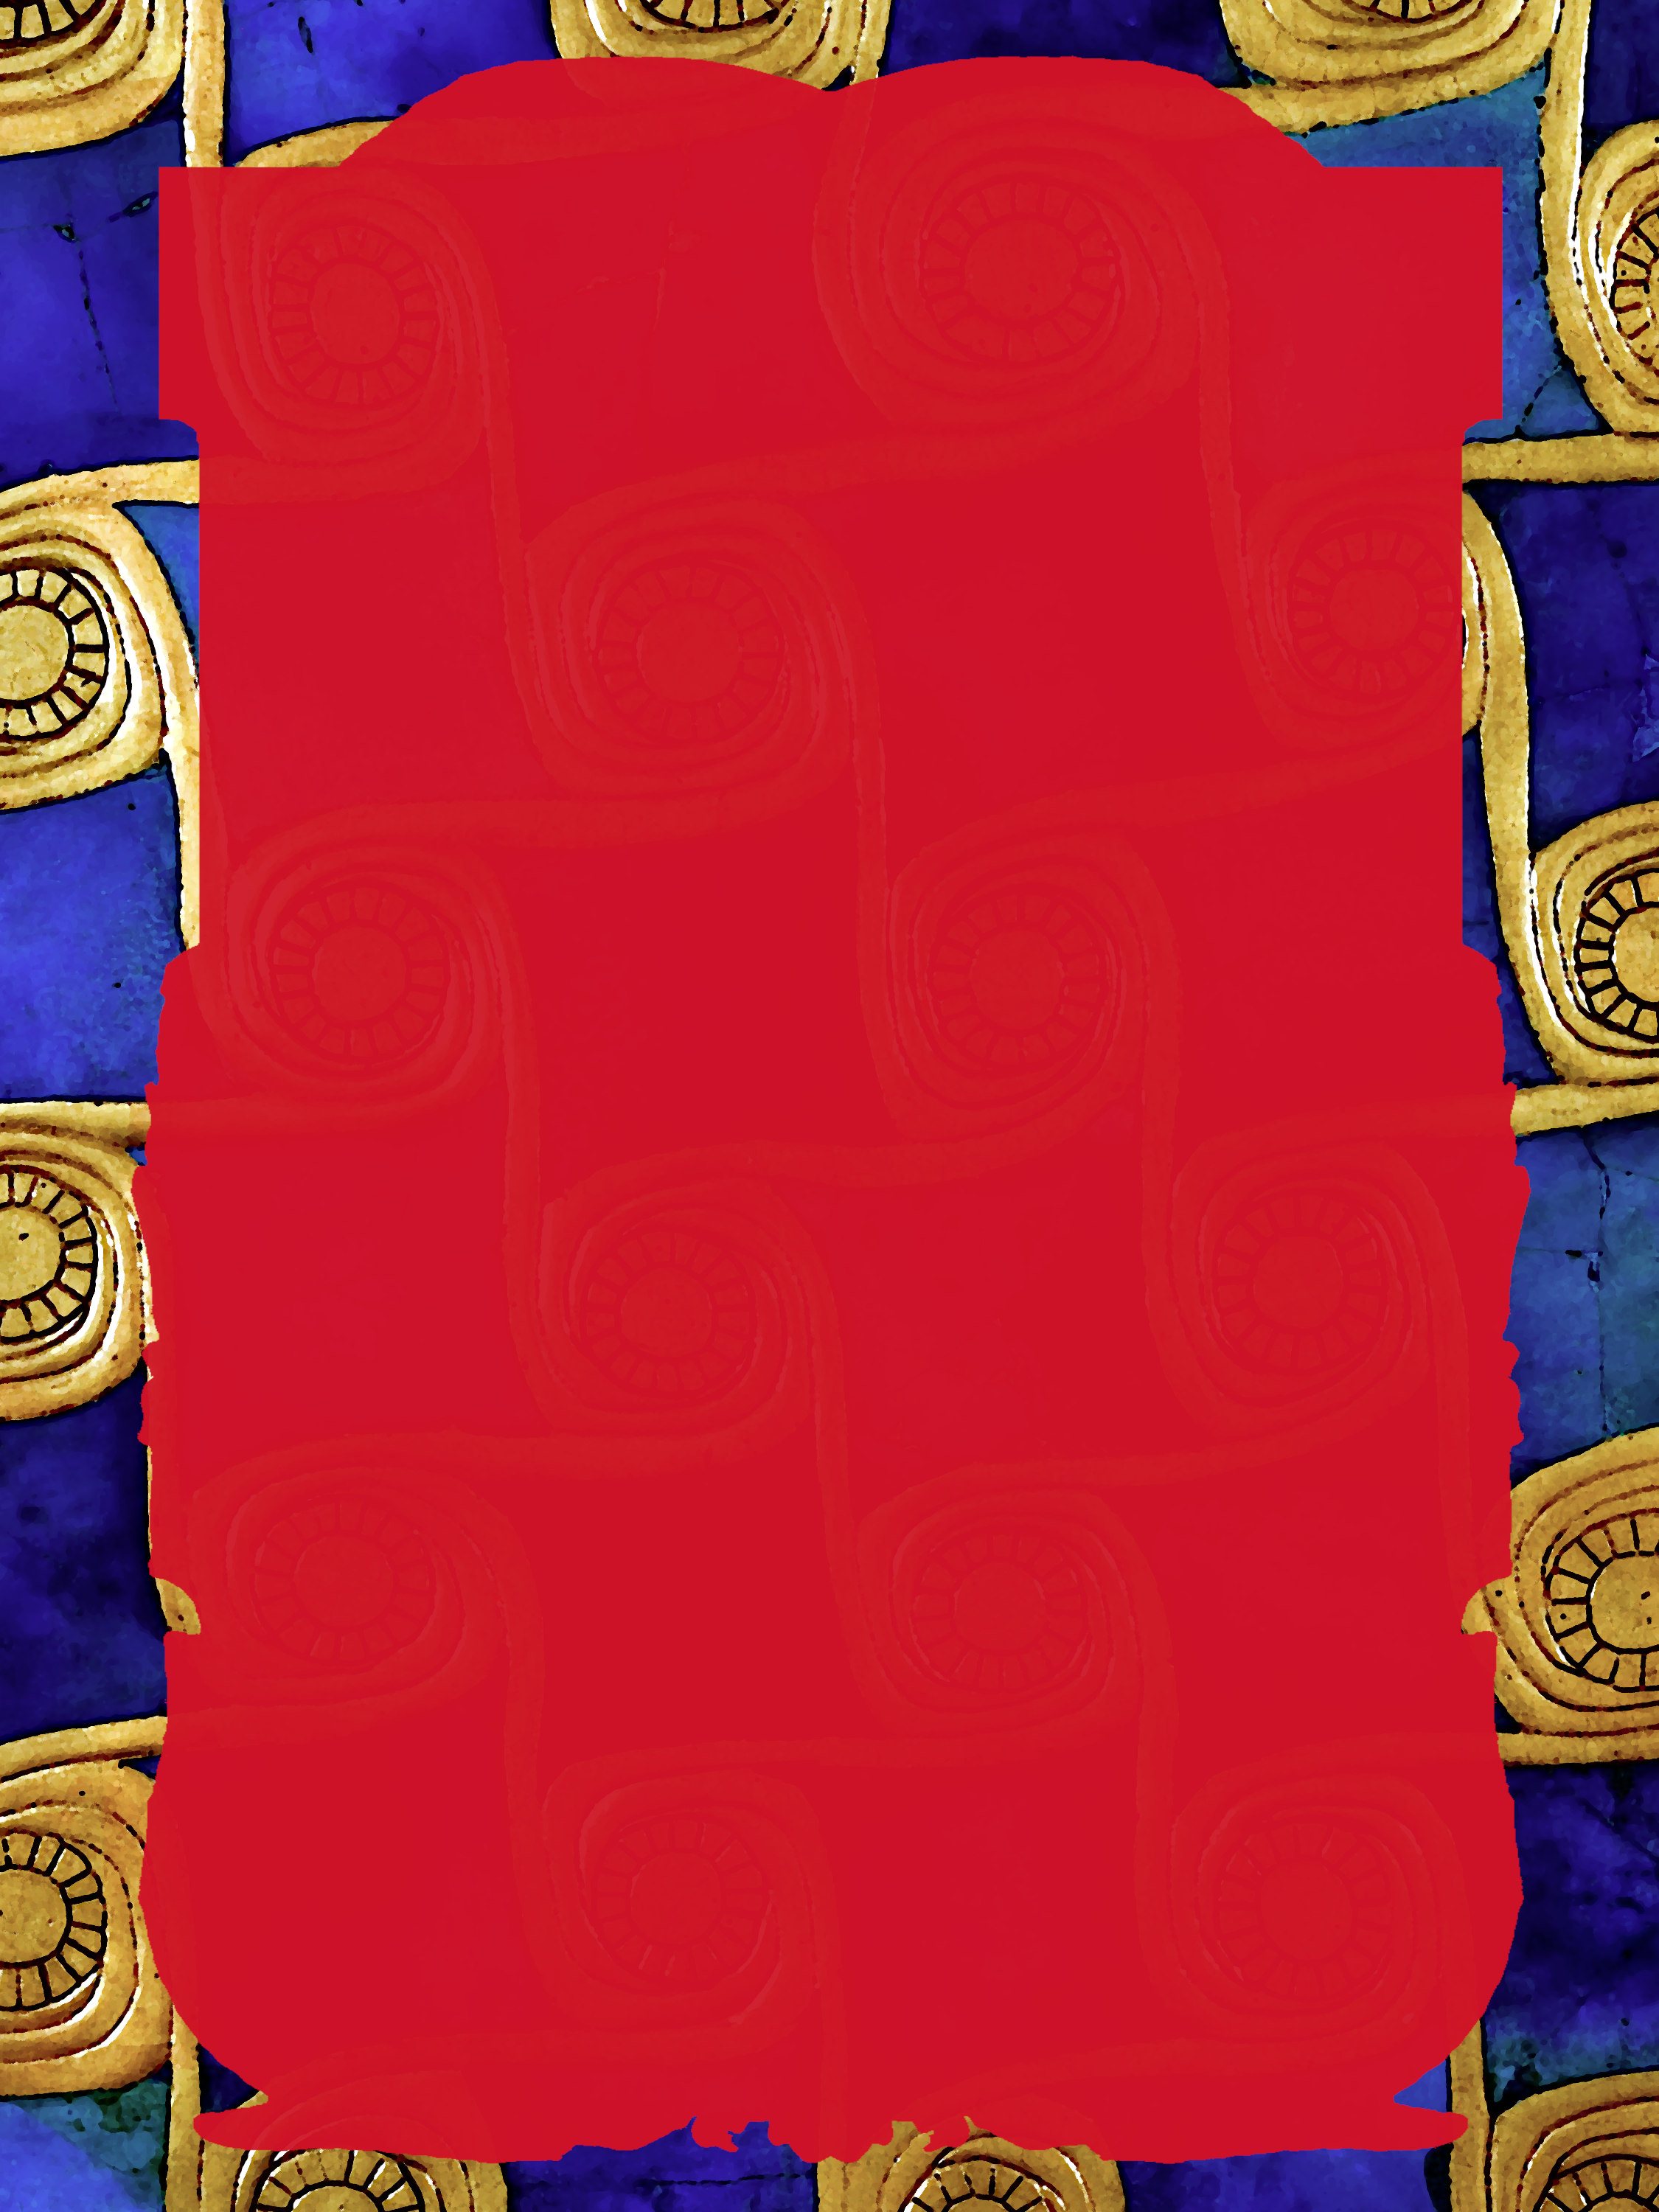
\includegraphics[width=\paperwidth,height=\paperheight]{ammon.jpeg}}
\begin{titlepage} % Suppresses headers and footers on the title page
	\centering % Centre everything on the title page
	%\scshape % Use small caps for all text on the title page

	%------------------------------------------------
	%	Title
	%------------------------------------------------
	
	\rule{\textwidth}{1.6pt}\vspace*{-\baselineskip}\vspace*{2pt} % Thick horizontal rule
	\rule{\textwidth}{0.4pt} % Thin horizontal rule
	
	\vspace{1\baselineskip} % Whitespace above the title
	
	{\scshape\Huge "Uber Meteorsteine.\\[1.25pt]}
	
	\vspace{1\baselineskip} % Whitespace above the title

	\rule{\textwidth}{0.4pt}\vspace*{-\baselineskip}\vspace{3.2pt} % Thin horizontal rule
	\rule{\textwidth}{1.6pt} % Thick horizontal rule
	
	\vspace{1\baselineskip} % Whitespace after the title block
	
	%------------------------------------------------
	%	Subtitle
	%------------------------------------------------
	
	{\Large\scshape Kongl. Vetensk. Acad. Handl. f. 1834.} % Subtitle or further description
	
	\vspace*{1\baselineskip} % Whitespace under the subtitle
	
    {\scshape\Large Von J. J. Berzelius.} % Subtitle or further description
    
	%------------------------------------------------
	%	Editor(s)
	%------------------------------------------------
    \vspace*{\fill}

	\vspace{1\baselineskip}

	{\Large\scshape Leipzig 1834.}
	
	{\Large\scshape{Verlag von Johann Ambrosius Barth.}}
	
	\vspace{0.5\baselineskip} % Whitespace after the title block

    \scshape\Large Internet Archive Online Edition  % Publication year
	
	{\scshape\Large Namensnennung Nicht-kommerziell Weitergabe unter gleichen Bedingungen 4.0 International} % Publisher
\end{titlepage}
\setlength{\parskip}{1mm plus1mm minus1mm}
\clearpage
\pagestyle{fancy}
\fancyhf{}
\cfoot{\swabfamily{\thepage}}
\tableofcontents
\clearpage
\LARGE
\section*{}
\paragraph{}
Erst seit Anfang dieses Jahrhunderts hat man es als wissenschaftlich bewiesen angesehen, dass von Zeit zu Zeit gr"o"sere und kleinere Steinmassen auf die Erde herabfallen, gew"ohnlich begleitet von einem stark krachenden donner"ahnlich rollenden Get"ose und einer Feuererscheinung, wobei der Stein auf seiner Oberfl"ache so schnell verglast wird, dass sein Inneres vor der ver"andernden Einwirkung der Hitze gesch"utzt bleibt. Gew"ohnlich zerspringt dadurch der Stein w"ahrend seines Falls und die St"ucke werden ziemlich weit umbergeschleudert. Wiewohl aus "alterer und neuerer Zeit dergleichen Steinf"alle beschrieben worden sind, so glaubte der besonnene Naturforscher doch lange die Zuverl"assigkeit solcher Nachrichten in Zweifel ziehen zu m"ussen, da kein annehmlicher Grund zu der Vermutung vorhanden war, den Ursprung so schwerer K"orper aus der Atmosph"are abzuleiten. Die sicherere Kenntnis, welche wir gegenw"artig zu besitzen glauben, ward begr"undet durch einen am 13. Dezember 1795 in England, zu Woldcottage in Yorkshire, sich ereignenden: und geh"orig beglaubigten Meteorsteinfall. Howard, der einige Jahre darauf eine Untersuchung dieses und mehrere anderer, angeblich vom Himmel gefallener Steine vornahm, fand sie im Ansehen und in der Zusammensetzung "ubereinstimmend, dagegen bestimmt verschieden von den Mineralien irdischer Abkunft. Als haupts"achlichstes Kennzeichen fand er, dass sie metallisches Eisen eingesprengt enthielten und dass dies Eisen nickelhaltig war. Howard teilte seine Untersuchung i. J. 1802 der K"onigl. Gesellschaft in London mit. Sie erregte allgemeine Aufmerksamkeit, wiewohl das von Howard aus seiner Untersuchung gezogene Resultat, welches von Pictet der franz"osischen Akademie der Wissenschaften mitgeteilt wurde, in der ersten Zeit f"ur einen Irrtum gehalten wurde. Der Zufall f"ugte es jedoch, dass sich wenige Monate darauf, am 26. Apr. 1803, zu L'Aigle im. Dép. de l’Orne einer der gr"o"sten und merkw"urdigsten Steinregen ereignete, wobei auf eine gewisse Fl"ache gegen ein Paar tausend Steinst"ucke ausges"ate wurden. Die Zahl der Augenzeugen war gro"s, und die franz"osische Akademie der Wissenschaften, schon aufmerksam geworden auf solche Ereignisse, "ubertrug ihrem Mitgliede Biot eine Untersuchung der Verh"altnisse an Ort und Stelle. Sein Bericht hob allen noch "ubrig gebliebenen Zweifel, dass die Steine von oben herabgefallen waren, und zwar unter Erscheinungen, die mit den von fr"uheren Meteorsteinf"allen angegebenen eine solche "Ahnlichkeit hatten, dass auch diese dadurch an Glaubw"urdigkeit gewannen.

Nun fing man an dar"uber nachzudenken, wo etwa diese fallenden K"orper entsprungen sein mochten. Die Vermutung, dass sie Ausw"urflinge irdischer Vulkane seien, bew"ahrte sich nicht, sowohl wegen der gro"sen Entfernung der Orte des Falls von Vulkanen als auch wegen der Verschiedenartigkeit der gew"ohnlichen vulkanischen Produkte. und der Meteorsteine. Man hat sie im Ernste als gebildet aus den Bestandteilen der Luft angesehen; allein wir wissen weder, ob die Bestandteile der Meteorsteine in Luftform existieren k"onnen, noch, ob sie aus den gew"ohnlichen Bestandteilen der Luft zusammengesetzt seien; und "uberdies, wenn dies auch der Fall w"are, haben doch mehre Meteorsteine eine se gro"se Masse gehabt, dass ihre Bildung im der Atmosph"are unm"oglich in der kurzen Zeit ihres Falles durch die Luft vor sich gehen konnte, besonders da notwendigerweise der Fall schon bei Absetzung des ersten festen Teilchens h"atte beginnen m"ussen.

Anaxagoras vermutete von einem zu seiner Zeit bei Aegos Potamos gefallenen Steine, dass er von einem anderen Weltk"orper ausgeworfen worden sei. Diese Ansicht schlie"st vermutlich die Wahrheit ein, und ist auch durch die Forschungen unserer Zeit unterst"utzt worden. Olbers "au"serte i. J. 1795 in einem Bericht "uber den am 16. Juli 1794 zu Siena in Italien geschehenen Meteorsteinfall die Idee, dass dergleichen Steine vom Monde ausgeworfen sein k"onnten, hielt es aber doch f"ur wahrscheinlicher, dass sie aus dem Vesuv herstammten. Im Jahr 1802 sprach Laplace, auf Veranlassung der Arbeit von Howard, dieselbe Idee aus, mit dem Zusatz, die Feuererscheinung entspringe aus der Zusammendr"uckung der Luft, in Folge der unendlichen Geschwindigkeit, mit welcher der Meteorstein in die Atmosph"are eindringe, welche aber durch den Widerstand der Luft so verringert werde, dass der Fall zuletzt nur mit der gew"ohnlichen Fallgeschwindigkeit geschehe.

Die uns zugewandte Seite des Mondes ist voller H"ohen, und darunter finden sich viele Berge, die den mit Kratern versehenen Vulkanen unserer Erde ganz "ahnlich gebildet sind, und dabei so gro"se Dimensionen haben, dass man mit guten Fernr"ohren in die Krater sehen und sehr wohl unterscheiden kann, dass die eine H"alfte der Innenseite von der Sonne beleuchtet und die andere beschattet ist, w"ahrend der Ring, welcher den Krater bildet, hervorsteht. Dies l"asst vermuten, dass diese Berge ihre Form durch dieselbe Ursache wie die auf der Erde erhalten haben, d. h. durch Eruptionen. Wenn aber die Kraft, welche auf dem Monde Eruptionen hervorbringt, eben so gro"s ist als die Wurfkraft der irdischen Vulkane, so m"ussen sich die geworfenen K"orper bedeutend weiter von dem Monde entfernen als von der Erde; denn erstlich ist die Masse des Mondes nur 1,45 Prozent von der der Erde, und damit steht auch die Schwere auf dem Mond im Verh"altnis; zweitens hat der Mond keinen Luftkreis, oder wenigstens einen: so lockeren, dass bei Fixsternbedeckungen durch den Mond keine Strahlenbrechung darin ‚wahrnehmbar ist. Der Auswurf geschieht folglich in einen luftleeren Raum, ohne einen solchen mechanischen Widerstand f"ur die Bewegung der geworfenen K"orper wie ihn die Atmosph"are der Erde darbietet, wo der K"orper daher. bald zur Ruhe kommt. Wenn drittens der Auswurf gegen die Erde gerichtet ist; so nimmt die Anziehung der Erde zu dem geworfenen K"orper best"andig zu, w"ahrend die des Mondes stetig abnimmt. Und viertens liegt die Gleichgewichtsgr"anze zwischen der Erde und dem Monde bedeutend n"aher am letzteren. Biot gibt an, dass eine Wurfkraft von 7771 Pariser Fu"s in der Sekunde diese Grenze erreiche; mit einem geringen Kraft"uberschuss wird der K"orper dieselbe "ubersteigen und dann auf die Erde fallen m"ussen. Diese Geschwindigkeit ist f"unf bis sechs Mal gr"osser als die einer 24 pf"undigen Kanonenkugel beim Austritt aus der Kanone, und wird von der Wurfkraft unserer Vulkane "ubertroffen.\footnote{\swabfamily{Laplace in v. Zachs Monatl. Korrespondenz, 1802 Septemb. S. 277.}} Die Berechnungen, welche sowohl Olbers\footnote{\swabfamily{Gilberts Annal. d. Physik, Bd. XV, S. 39.}} als Poisson\footnote{\swabfamily{Ebendaselbst, S. 329.}} hier"uber angestellt haben, zeigen, dass die Idee eine physische M"oglichkeit einschlie"se.

Verschiedene Umst"ande bei den Meteorsteinen passen wohl zu dem, was wir glauben von dem Monde zu wissen. Die Meteorsteine sind durchsetzt mit metallischem Eisen, welches, wenn der Stein mit lufthaltigem Wasser befeuchtet wird, allm"ahlig zu Eisenoxydhydrat rostet wie es unter gleichen Umst"anden mit den Mineralien der Erdkruste der Fall ist. In ihrer urspr"unglichen Lagerst"atte mangelt also Luft, oder beides, Luft und Wasser. Auch haben astronomische Untersuchungen keine Spur von so gro"sen Wasseransammlungen auf dem Mende gefunden, dass sie mit guten Fernr"ohren zu entdecken w"aren. Ich wei"s nicht, dass man in den Meteorsteinen chemisch gebundenes Wasser gefunden habe. --- Wir werden in der weiterhin folgenden Untersuchung finden, dass die meisten Meteorsteine einander in der Zusammensetzung so "ahnlich sind, dass man sie als von demselben Berg herr"uhrend ansehen kann, w"ahrend nur wenige von abweichender Beschaffenheit gefunden wurden. Soweit es zul"assig ist, aus den Verh"altnissen auf der Erde einen Schluss zu ziehen, kann man die "ubrigen Weltk"orper auch gar nicht als homogene Gemenge von Mineralien ansehen, vielmehr hat die Geschichte ihrer urspr"unglichen Bildung sicher viele "Ahnlichkeit mit der Geschichte der der Erde. Die Felsarten aus verschiedenen Gegenden eines anderen Weltk"orpers werden also in der Zusammensetzung verschieden sein k"onnen.

Der Mond kehrt der Erde best"andig dieselbe Seite zu. Der Mittelpunkt seiner siebtbaren Scheibe macht folglich deren best"andig uns zugewandten Gipfel aus, dessen Eruptionen ihre Projektile am leichtesten "uber die Gleichgewichtslinie hinauswerfen, und folglich m"ussen die auf die Erde fallenden Meteorsteine, angenommen, dass sie vom Monde kommen, in gr"o"ster Zahl von hier ab ausgeworfen worden sein. Sie k"onnen folglich einem ganz beschr"ankten Gebirgszug angeh"oren, und dann l"asst sich ihre gro"se Gleichheit im Ansehen und in der Zusammensetzung leicht begreifen. Die Ausw"urflinge von Eruptionen, welche seitw"arts dieses Gipfels geschehen, fliegen in einer nicht mehr direkt gegen die Erde gerichteten Linie fort, und m"ussen also seltener in den Anziehungskreis der Erde gelangen. Wenn die Bergarten dieser Gegenden verschieden sind von denen auf dem Gipfel der uns zugewandten Mondesh"alfte, so sieht man leicht ein, dass uns von daher Meteorsteine von anderer als der gew"ohnlichen Beschaffenheit zukommen m"ussen, zugleich aber auch, dass dies vergleichungsweise selten geschehen m"usse. Darf man annehmen, dass der uns zugewandte Mondsscheitel so mit Nickeleisen ‚durchsetzt ist als es die Meteorsteine sind, und dass die "ubrigen Teile, oder wenigstens die best"andig von’ der Erde abgewandte Halbkugel, wenig oder gar nichts davon enthalten, so w"urde daraus folgen, dass der Mond, wenn auf ihn die Erde, au"ser ihrer allgemeinen, von der Schwere herr"uhrenden Anziehung, noch eine magnetische Anziehung aus"ubte, den eisenreichsten Teil seiner’ Kugel gegen die Erde wenden m"usse, und dass daraus die wunderbare Erscheinung entstehe, dass der Mond uns unverwandt die n"amliche Seite zukehrt.

Es ist jedoch auch m"oglich, dass die Meteorsteine von einem anderen kosmischen Orte herkommen. Olbers "au"serte bekanntlich die Vermutung, dass die kleinen Planeten zwischen Mars und Jupiter St"ucke eines zersprungenen Planeten sein k"onnten, in Folge weicher Vermutung mehre dergleichen St"ucke. gesucht wurden, und Olbers selbst eines derselben fand. Wem eine solche Katastrophe stattfand, was durch den bedeutenden Winkel, welchen die Bahn der Pallas mit den Bahnen der "ubrigen Planeten macht, best"atigt zu werden scheint, so muss eine unendliche Menge kleiner St"ucke umhergeschleudert worden sein in Richtungen, dass sie um die Sonne abnehmende Bahnen beschreiben, wodurch sie dann leicht auf ihrem Wege in die Attraktionssph"are anderer Planeten geraten und auf sie niederfallen. Man hat auch vermutet, die Materie des Weltalls befinde sich zum Teil in einer noch nicht geordneten Bewegung und die Meteorsteine seien solche mehr oder weniger gro"se Massen‚ welche zuweilen in die Attraktionssph"are der Erde geraten; allein diese Vermutung ist von allen die wenigste wahrscheinliche. Das Weltsystem scheint von der bestimmtesten Ordnung zu zeugen, und "uberdies wird ‚nach dieser Vermutung die identische Beschaffenheit der Meteormassen noch weniger begreiflich.

Indes l"asst sich als ausgemacht ansehen, dass sie nicht von der Erde, sondern von einem anderen Weltk"orper herstammen, und folglich die Beschaffenheit der au"serhalb der Erde vorkommenden w"agbaren Stoffe verk"unden. In dieser Beziehung haben die Meteorsteine ein au"serordentliches Interesse. Von Wichtigkeit dabei ist es, nicht nur die Mineralien, aus denen sie bestehen, auszumitteln, sondern auch die geringste Spur von zuvor noch nicht darin gefundenen Elementen. M"oglich w"are es, darunter solche zu finden, welche noch nicht auf der Erde angetroffen sind.

Wie stark auch die Vermutung im Voraus war, dass die Schwerkraft im ganzen Universum herrsche, so haben doch die Astronomen mit besonderem Interesse in den Uml"aufen der Doppelsterne umeinander eine Wirkung derselben Gravitationsgesetze erkannt, welche f"ur unser Planetensystem g"ultig sind. Nicht minder interessant ist es zu erfahren, aus welchen Stoffen andere Weltk"orper bestehen, und die Gewissheit zu erlangen, dass sie von einerlei Natur mit denen sind, welche die Masse der Erde ausmachen. Haben wir gleich die letzteren noch nicht alle in den Metvorsteinen aufgefunden, so haben wir doch einen gro"sen Teil der allgemeiner verbreiteten darin angetroffen, und wir werden in dem Folgenden sehen, dass es gegl"uckt ist zu bestimmen, in welchen chemischen Verbindungen sie darin enthalten sind.

Die Arbeit "uber Meteorsteine, welche ich hier die Ehre habe der K. Akademie zu "uberreichen, ist veranlasst worden durch eine Aufforderung, den am 25. November 1833, um 6 1/4 Uhr Abends in der Nachbarschaft von Blansko in M"ahren niedergefallenen Meteorstein chemisch zu untersuchen. Er bildete wie gew"ohnlich ein stark leuchtendes Feuerph"anomen und seinem Falle ging ein donner"ahnliches Get"ose voran. Der Bergamts-Direktor Reichenbach, welcher sich damals auf dem Felde befand und Zeuge des Meteors war, stellte hernach mit ‚einer starken Mannschaft eine Aufsuchung der gefallenen Masse an, und dadurch gl"uckte es endlich, kleine St"ucke, zum Belauf von etwa einem halben Pfunde aufzufinden, aber die Hauptmasse zu entdecken gelang, haupts"achlich wegen, der waldigen Beschaffenheit dieser Gegend, noch nicht.

\section{\swabfamily{Meteorstein von Blansko.}}
\paragraph{}
Dieser Meteorstein geh"ort zu den h"aufigste vorkommenden, und kann, neben einem derselben gelegt, z. B. neben den von Benares, l’Aigle, Berlougville, u. s. w., von ihm nicht unterschieden werden. Seine Beschreibung ist folglich die Beschreibung von diesen. Er hat die gew"ohnliche, "au"serlich geschmolzene Rinde, eine hellgraue, etwas rostfleckige, feink"ornige Bruchfl"ache, die hie und da runde K"ugelchen von gleicher Farbe mit dem Steine zeigt; letztere k"onnen ausgel"ost werden und hinterlassen dann eine glatte H"ohlung. Er enth"alt viel Nickeleisen, und sehr wenig Schwefeleisen, in feinen Partien "uberall eingesprengt, und dadurch zeigt er gl"anzende Punkte, von denen einige in einer gewissen Richtung r"otlich erscheinen, indes doch nichts anderes sind als angelaufenes Nickeleisen. Zerst"o"st man den Stein zu einem gr"oblichen Pulver, so kann das Nickeleisen mit einem Magneten ausgezogen, und unter Wasser von der sichtlich anh"angenden Steinsubstanz abgewaschen werden, so dass die Eisenteilchen fast silberwei"s zur"uckbleiben. Indes schlie"sen dieselben doch in ihren Vertiefungen und H"ohlungen noch viel Steinsubstanz ein, welche bei Aufl"osung des Eisens teils zersetzt, teils abgelagert wird. In dem zu meinen Versuchen angewandten St"ucke waren 17,15 Prozent Nickeleisen, von denen die eingeschlossene Steinmasse bereits abgerechnet ist. Unter einem zusammengesetzten Mikroskop kann man mit Deutlichkeit keine anderen Bestandteile unterscheiden als ein wei"ses splittriges Mineral, welches scheint durchscheinend zu sein und bei den R"ostflecken gelblich ist, und die metallischen kantigen K"orner. Dasselbe ist der Fall, wenn man das gr"obliche Pulver des Minerals unter dem Mikroskop betrachtet; allein dann sind seine Teile durchsichtiger.

Auf mechanischem Wege habe ich aus dem Meteorstein nichts anderes abscheiden k"onnen als das wei"se Mineral, die runden K"ugelchen und Nickeleisen. Auf chemischen Wege habe ich abgeschieden: Nickeleisen, Schwefeleisen, Chromeisen, ein wei"ses Mineral, welches von S"auren zerlegt wird, und ein "ahnliches, welches von S"auren nicht angegriffen wird. Obgleich der Stein ziemlich gleichf"ormig gemengt zu sein scheint, so ist doch ganz deutlich das Nickeleisen an gewissen Stellen reichlicher als an andern zugegen. Gewisse Teile des Steins geben beim Reiben ein dunkleres Pulver als andere.

Dor nicht magnetische Teil des Steins verh"alt sich vor dem L"otrohr folgenderma"sen: Er gibt, gelinde gegl"uht, kein Wasser und ver"andert sich nicht. Wird ein St"uck an offener Luft gebrannt, so ist der Geruch nach schwefliger S"aure erkennbar, und der Stein wird obenauf schwarz, inwendig rotfleckig. Das Pulver des Steins brennt sich im Gl"uhen rot, und schmilzt endlich, aber weit tr"ager als Feldspat, zu einer schwarzen Glaskugel mit matter Oberfl"ache, ganz "ahnlich der schwarzen Rinde, welche den Stein von au"sen umgibt. Von Borax wird er leicht zu einem eisengr"unen Glase gel"ost; ebenso vom Phosphorsalz, jedoch mit Hinterlassung eines Kieselskeletts. Mit kohlensaunen Natron schmilzt der Stein zu einer schwarzen Kugel. Dies ist das, gew"ohnliche Verhalten der Meteorsteine vor dem L"otrohr.

Ich werde diese Untersuchung in zwei Hauptabschnitte teilen, n"amlich 1. von den nicht magnetischen, und 2. von den mit dem Magneten ausziehbaren Teilen handeln.

Diese mechanische Abscheidung durch den Magneten scheint zwar ganz leicht zu sein l"asst sich aber doch so gut wie unm"oglich ganz vollst"andig bewirken. Das Schwefeleisen verwandelt sich beim Reiben in Pulver, welches sich unterschiedslos dem Steinpulver beimengt und ihm eine dunklere Farbe erteilt. Um erst das meiste auszuziehen stie"s man den Stein zu grobem Pulver, und zog aus diesem das Magnetische unter Wasser aus. Als dem Magneten nichts mehr folgen wollte, rieb man den R"uckstand zu feinem Pulver und behandelte dasselbe abermals unter Wasser mit dem Magneten, wodurch an wieder eine kleine Portion magnetischer Teile erhielt. Den R"uckstand zerrieb man nun in einer Porphyrschale und schlemmte ihn. Das trockne Pulver war hellgrau und rot, bei "Ubergie"sung mit Salzs"aure, nach Schwefelwasserstoffgas, und, beim Gl"uhen, nach schwefliger S"aure, beide Mal schnell vor"ubergehend, aber doch die Gegenwart einer Portion Schwefeleisen beweisend, die vom Magneten nicht ausgezogen worden war.

Zur Vermeidung unn"otiger Weitl"aufigkeiten werde ich ein f"ur alle Mal den beiden Analysen eingeschlagenen Weg beschreiben und sodann, bei jeder einzelne Art, wo nicht von diesem Wege abgewichen wurde, nur das Resultat anf"uhren.

A. Das Steinpulver wurde in einem Platingef"a"s mit konzentrierter Salzs"aure zersetzt; es entstand dadurch eine Gelatinirung, die aber doch nur partiell war. W"ahrend der Zersetzung war das Gef"a"s mit einem reinen Uhrglase bedeckt; dies wurde aber nicht angegriffen, zeigte also die Abwesenheit von Fluorverbindungen an. Die Masse wurde eingetrocknet, mit Salzs"aure befeuchtet und nach einer Weile mit Wasser ausgezogen. Das Ungel"oste wurde ausgewaschen, noch feucht zwei Mal mit kohlensaurem Natron gekocht, die L"osung jedesmal mit vielem kochenden Wasser verd"unnt und dann noch siedend hei"s filtriert. Das Gewicht des nun Ungel"osten gab den Gehalt des Meteorsteins an in S"auren unl"oslichen Verbindungen, und, durch Subtraktion von dem Gewicht der angewandten Menge, auch die Menge dies durch S"auren zerlegten Teils des Minerals. Die L"osung in kohlensaurem Natron wurde mit Salzs"aure "ubers"attigt und im Wasserbade zur Trockne verdunstet, bei Wiederaufl"osung in Wasser blieb die Kieselerde des von der S"aure zersetzten Minerals zur"uck. Die L"osung in Wasser wurde mit Ammoniak gepr"uft, dass sie keinen Niederschlag gab, und das Waschwasser von der Kieselerde wurde zur Trockne verdunstet, worauf der R"uckstand, bei Behandlung mit Wasser, noch etwas Kieselerde hinterliefs, welche das Wasser w"ahrend des Auswaschens aufgenommen hatte.

B. Die L"osung: des zersetzten Minerals in Salzs"aure wurde mit Salpeters"aure oxydiert, die L"osung mit "atzendem Ammoniak gef"allt, um in der Fl"ussigkeit neben einem Teil der Talkerde, Kalk und Alkali zur"uckzuhalten. Als ich nun die Fl"ussigkeit sogleich mit kohlesaurem Ammoniak niederschlage, erhielt ich immer weniger Kalk als wirklich im Stein vorhanden war. Ich fand bemach, aber zu sp"at, um noch Gebrauch davon machen zu k"onnen, dass der Plan der Analyse fehlerhaft war, da n"amlich der Meteorstein Zinnoxid enthielt, weiches vor der Oxydation mit Salpeters"aure h"atte durch Schwefelwasserstoff gef"allt werden m"ussen. Indes ist die Menge der Zinnoxyds so gering, dass es ganz vernachl"assigt werden kann, nachdem man wei"s, dass es sich darin befindet.

Die mit "atzendem Ammoniak gef"allte Fl"ussigkeit wurde mit etwas Schwefelwasserstoff-Schwefelammonium versetzt (wodurch sie schwarz ward), und damit in einer verkorkten Flasche stehen gelassen, bis sie, mit einem Stich ins Gelbe, klar geworden war. So lange die klar gewordene Fl"ussigkeit farblos ist, kenn man nicht sicher sein den ganzen Nickelgehalt ausgef"allt zu haben. Zur Kl"arung sind oft 24 Stunden erforderlich. Diese Methode zur Abscheidung des Nickeloxyde ist die beste, welche ich kenne. Indes hat sie doch zwei Fehler. Der eine besteht darin, dass beim Waschen etwas schwefelsaures Nickeloxyd wieder gebildet wird, und der andere, dass durch wechselseitige Verwandtschaft etwas Schwefelmagnesium entsteht und sich mit dem Schwefelnickel niederschl"agt, besonders wenn das Gemenge zum Kl"aren in die W"arme gestellt wird. Indes haben die Fehler der Methode keinen wesentlichen Einfluss auf das Resultat der Analyse Um aus dem Schwefelmetall die Menge des Nickeloxyds zu bestimmen, ward es ger"ostet, in Salzs"aure gel"ost, mit "atzendem Kali gef"allt und gewaschen, gew"agt und gegl"uht. Das so erhaltene Nickeloxyd enthielt bei allen Versuchen Kupferoxyd, wie es sich vor dem L"otrohr durch die gew"ohnliche Reduktion zu Kupferoxydul nachweisen lie"s. Es zeigte noch ein anderes Verhalten, welches meine Aufmerksamkeit erregte; es gab n"amlich, eingeschmolzen in Phosphorsalz und mit der Oxydationsflamme beblasen, ein Glas, welches keim Erkalten undurchsichtig und farblos ward. Die Veranlassung davon war, wie es sodann zeigte, ein Gehalt von Zinnoxid. Wird das Nickeloxyd mit Phosphorsalz geschmolzen, metallisches Zinn hinzugesetzt und dann so stark darauf geblasen, dass sowohl das Nickel als das Kupfer im reduzierten Zustand vom Zinn aufgenommen wird, so erh"alt man beim Erkalten ein tr"ubes Glas von blassblauer Farbe, was einen geringen Gehalt von Kobalt im Nickeloxyd andeutet. Nachdem das Zinn als best"andiger Bestandteil der Meteorsteine aufgefunden worden, "anderte ich die Operationsmethode dahin ab, dass ich die L"osung in Salzs"aure erst mit Schwefelwasserstoffgas f"ullte, den "Uberschuss desselben durch Abdunsten der filtrierten Fl"ussigkeit entfernte und darauf die Fl"ussigkeit im konzentrierten Zustand zum Behufe der Oxydation des Eisens auf die im "Ubrigen zu Anfange von B angef"uhrte Weise mit etwas Salpeters"aure vermischte.

C. Die mit Schwefelwasserstoff-Schwefelammonium gef"allte Fl"ussigkeit wurde mit oxalsauren Ammoniak auf Kalk gepr"uft, gew"ohnlich aber von diesem nicht die geringste Spur erhalten. Da nach mehreren Stunden keine Tr"ubung bemerkt wurde, dunstete ich die Fl"ussigkeit im Wasserbade zur Trockne ein, erhitzte den R"uckstand vorsichtig in einer Porzellanschale bis zur Zersetzung des salpetersauren Ammoniaks, dann bis zur Verjagung des Salmiaks, und nun "uber einer Weingeistflamme bis zam gelinden Gl"uhen der Schale, solange noch ein Geruch nach Salzs"aure versp"urt werden konnte. Nach dem Erkalten der Schale wurde die Masse mit "atzendem Ammoniak befeuchtet, mit Wasser ausgezogen und die Talkerde auf ein Philtrum gebracht. Gew"ohnlich ward sie, in Folge eines Mangangehalts, beim Gl"uhen rosenrot, Die L"osung wurde im Platintiegel zur Trockne verdunstet, der Salmiak verjagt und der Boden des Tiegels bis zum anfangenden Gl"uhen erhitzt, dann ein zu einer Kugel aufgerolltes und mit destilliertem Wasser befeuchtetes Philtrum hineingeworfen und der Deckel aufgelegt. Der Zweck hierbei war, das r"uckst"andige Chlormagnesium in einer Atmosph"are von Wassergas zu erhitzen, um allen Chlorgehalt v"ollig fortzunehmen. Nachdem das Papier sich verkohlt hatte, lie"s ich den Tiegel erkalten, nahm die Papierkohle heraus, oder verbrannte sie, wenn sie festgeklebt war. Das Wasser zog nun Chlor-Alkalium aus, welches, nach Verdunstung des Wassers zur Trockne, gewogen wurde. Durch Zusatz von Platinchlorid, Abdunstung des Salzes und Behandlung desselben mit Alkohol wurde der Gehalt an Chlorkalium darin auf die gew"ohnliche Weise bestimmt. Die im Tiegel festsitzende, von Kohle geschw"arzte Talkerde wurde wei"s gebrannt und gew"agt.

D. Das in B mit "atzendem Ammoniak Gef"allte wurde in Salzs"aure gel"ost und mit kohlensaurem Ammoniak niedergeschlagen, weil ich fand, dass "atzendes Kali keine Tonerde daraus zog, ehe diese neue F"allung vor sich gegangen war. Nun blieb sehr viel Talkerde in der Losung zur"uck, aus der sie auf die gew"ohnliche Weise erhalten wurde. Sie enthielt gew"ohnlich eine geringe Spur von Nickeloxyd.

Aus dem mit kohlensaurem Ammoniak erhaltenen Niederschlag zog "atzendes Kali Tonerde aus, doch immer nur sehr wenig, welche dann auf gew"ohnliche Weise abgeschieden wurde.

Der so behandelte R"uckstand wurde in Salzs"aure gel"ost und bei Digestion auf einem Wasserbade mit bernsteinsaurem Ammoniak gef"allt, wodurch Eisenoxyd abgeschieden wurde.

Aus der so gef"allten Fl"ussigkeit wurde mit kohlensaurem Kali, nach Zersetzung der Ammoniaksalze und Verjagung des Ammoniaks, Nickeloxyd erhalten, welches Talkerde und etwas Manganoxyd enthielten. Talkerde und Nickeloxyd zu trennen ist "au"serst schwer, und l"asst sich unm"oglich mit vollst"andiger Genauigkeit bewirken. Nachdem ich gefunden, dass oxalsaures Ammoniak, so wie das L"osen in Essigs"aure und Behandeln der durch Ammoniak neutralisierten L"osung mit Schwefelwasserstoffgas kein gen"ugendes Resultat lieferte, bediente ich wich der Digestion des gegl"uhten Oxyds mit verd"unnter Salpeters"aure, wobei das Oxyd meist ungel"ost zur"uckblieb, f"ullte die L"osung mit Schwefelwasserstoff-Schwefelammonium, filtrierte sie, trocknete sie ein, und brannte die Salpeters"aure fort, um die Talkerde zu erhalten, deren Gewicht von dem gemeinschaftlichen des Nickeloxyds und der Talkerde abgezogen wurde. Nickelfrei wurde zwar die Talkerde auf diese Weise nicht erhalten; allein die Spur, welche sie von diesem zur"uckhielt, hatte keinen wesentlichen Einfluss auf das Resultat. Die Talkerde ist nach dem Gl"uhen von einem andern gebrannten wei"sen R"uckstand daran zu erkennen, dass sie beim ger"oteten Lackmuspapier die blaue Farbe wieder herstellt.

E. Der in A unl"osliche Teil des Meteorsteins, welches erst mit Salzs"aure und dann kochend mit kohlensaurem Natron behandelt worden, wurde bei verschiedenen Versuchen auf dreierlei Weisen behandelt, n"amlich entweder mit kohlensaurem Baryt oder kohlensaurem Natron gegl"uht, oder auch mit Fluorwasserstoffs"aure behandelt.

Gl"uhen mit kohlensaurem Baryt. Die gegl"uhte Masse, weiche der starken Hitze eines Kohlenofens ausgesetzt worden, war nicht geschmolzen. Ihre Farbe war grau geworden. Sie gelatinierte wie gew"ohnlich mit Salzs"aure. Die Kieselerde wer im feuchten Zustand dunkelgrau, im trocknen aber wei"s. Nach Aufl"osung durch Kochen mit kohlensaurem Natron blieb ein schwarze Pulver zur"uck, welches sich nicht weiter l"osen wollte, und nach dem Trocknen braun wurde. Dieses Pulver ergab sich vor dem L"otrohr als Chromeisen, welches in dieser analytischen Methode eine Zersetzung erlitt; als es aber in Phosphorsalz aufgel"ost wurde, zeigte es zwei Eigenheiten, n"amlich dass metallisches Platin aus der Oberfl"ache der Kugel herauskroch und dass die klare Kugel beim Erkalten tr"ube gr"un ward. Das Platin r"uhrte sichtlich im Versuche von dem Platintiegel her, welcher bei dem Gl"uhen schien angegriffen worden zu sein. Ich w"urde dieses Umstandes gar nicht erw"ahnt haben, wenn ich nicht einen ganz gleichen bei der Zerlegung des Minerals durch Fluorwasserstoffs"aure beobachtet h"atte, wiewohl hier kein Anfressen des Tiegels merkbar war. Indes habe ich doch keinen Grund, dieses Platin von etwas anderem als dem gebrauchten Platintiegel herzuleiten. Den Bestandteil, welcher die Phosphorsalzkugel tr"ubte, stellte ich auf folgende Weise dar. Das Chromeisen wurde durch Schmelzen mit saurem schwefelsauren Kali aufgel"ost, wobei das Platin obenauf floss und einen Teil der Oberfl"ache versilberte, wo es sich w"ahrend des Abk"uhlens erhielt und abgenommen werden konnte. Die Masse wurde in Wasser gel"ost und durch die schwach gr"une L"osung ein Strom von Schwefelwasserstoffgas geleitet; es entstand dadurch ein gelbbrauner Niederschlag, welcher, nach dem R"osten, mit kohlensaurem Natron und Borax im Reduktionsfeuer behandelt, ein geschmeidigeres Zinnkorn gab. Mit Phosphorsalz konnte darin ein geringer Kupfergehalt entdeckt werden. Das schwarze Pulver war also Chromeisen, welches eine verh"altnism"a"sig sehr geringe Menge Zinnoxid enthielt, wahrscheinlich im Zustand des gew"ohnlichen Zinnsteins.

Die L"osung der gegl"uhten Steinmasse in Salzs"aure wurde durch Schwefels"aure vom Baryt, und durch Schwefelwasserstoff-Schwefelammonium vom Nickeloxyd befreit, mit Salpeters"aure oxydiert und abgeraucht, so dass die Schwefels"aure sowohl alle Salpeters"aure als Salzs"aure aus jagte, wieder in Wasser gel"ost, mit "atzendem Ammoniak gef"allt, darauf die in der Fl"ussigkeit zur"uckgeblieben Alkalien nebst dem Kalk und der Talkerde auf gew"ohnliche Weise, d. h. mit essigsaurem Baryt, abgeschieden, was im Detail anzugeben mir "uberfl"ussig scheint.

Der Niederschlag mit "atzendem Ammoniak wurde wieder in Salzs"aure gel"ost und mit kohlensaurem Ammoniak gef"allt; dabei blieb die Talkerde in der Fl"ussigkeit zur"uck, aus welcher sie gef"allt und ihrem Gewichte nach bestimmt wurde.

Der Niederschlag gab mit "atzendem Kali Tonerde. Aus der Fl"ussigkeit, aus welcher die Tonerde mit kohlensaurem Ammoniak gef"allt war, wurde durch Abdunsten und durch Gl"uhen mit Salpeter eine deutliche Spur von Chrom erhalten, welche sich mit salpetersaurem Bleioxyd f"allen liefs, aber doch nicht das W"agen verdiente.

Das mit "atzendem Kali behandelte Eisenoxyd aufs Neue gel"ost und mit bernsteinsaurem Ammoniak gef"allt, liefs etwas Nickeloxyd mit Talkerde in der Fl"ussigkeit zur"uck. Sie wurden auf vorhin genannte Weise geschieden.

Der Niederschlag mit bernsteinsaurem Ammoniak wurde gegl"uht und gewogen, dann zum feinsten Pulver gerieben und in einem Platintiegel mit Salpeter und etwas kohlensaurem Kali gebrannt. Die gelbe Salzmasse wurde mit Wasser ausgekocht, die L"osung mit Essigs"aure ges"attigt und gef"allt zuweilen mit salpetersaurem Quecksilberoxydul, wo dann der gegl"uhte Niederschlag Chromoxyd war, oder zuweilen mit salpetersaurem Bleioxyd, was chromsaures Bleioxyd gab. Aus beiden Niederschl"agen wurde der entsprechende Gehalt an Chromeisen nach der Formel FeCr berechnet. Da das gemeinschaftliche Gewicht des Eisen- und Chromoxyds bekannt war, wurde das des Eisenoxyds durch Abzug des vom Chromoxyd erhalten. Das Eisenoxyd wurde zu Oxydul berechnet, und davon die Menge abgezogen, welche n"otig war, um mit dem Chromoxyd Chromeisen zu bilden.

Bei der Analyse des: l"oslichen wie des unl"oslichen Teils der Bergart des Meteorsteins bestimmte ich den, Mangangehalt auf die Weise, dass ich alle erhaltene Talkerde sammelte, gl"uhte und wog, darauf in Salzs"aure l"oste, und zu dieser L"osung, nachdem sie in eine Flasche gegossen war, ein Gemenge von chlorigsaurem und doppelt kohlensaurem Natron gro"s; das Mangan fand sich dann nach 24 Stunden als Oxyd gef"allt, welches nun gegl"uht, gewogen und von dem Gewichte der Talkerde abgezogen ward.

Das Gl"uhen mit kohlensaurem Natron geht am besten, wenn man nicht beabsichtigt, das Chromeisen in Substanz abzuscheiden und die geringe Menge Alkali zu bestimmen. Auch bei dieser Methode bekommt man in dem mit bernsteinsaurem Ammoniak gef"allten Eisenoxyd einen Hinterhalt von Chromoxyd.

Die Analyse durch Fluorwasserstoffs"aure geht leicht. Nachdem die S"aure im Wasserbade ab ged"unstet ist, setzt man Schwefels"aure hinzu und vertreibt die Flusss"aure aus dem R"uckstand. Die Masse ist schwarz von unaufgel"ostem Chromeisen, welches nach Verd"unnung der L"osung mit Wasser und nach Digestion zur Aufl"osung des Gipses zur"uckbleibt. In "Ubrigen geschieht die Analyse ganz so wie bei der mit Baryt, nachdem dieser durch Schwefels"aure gef"allt worden ist. Der Gehalt an Kieselerde gibt sich ‚durch den Verlust zu erkennen. Auch hier findet man, au"ser der Tonerde, eine Spur von Chrom vom "atzenden Kali ausgezogen, und in dem mit bernsteinsaurem Ammoniak gef"allten Eisenoxyd gleichfalls eine Portion Chromoxyd.

Der Meteorstein von Blansko dieser Behandlung unterworfen, gab von dem durch S"auren zersetzbaren Minerale 51,5, von dem in S"auren unl"oslichen 48,5. In einem anderen Versuch wurden 48,9 vom ersteren und 51,1 vom letzteren erhalten, woraus zu folgen scheint, dass das Gemenge nicht vollkommen homogen an allen Punkten ist.

Die Analyse des l"oslichen Minerals, auf 100 Teile berechnet, gab folgende Bestandteile:
\begin{center}
\begin{tabular}{ |l|r|r| }
    \hline
     & & Sauerstoff\\\hline
    Kieselerde & 33,084 & 17,192\\\hline
    Talkerde & 36,143 & 14,00\\\hline
    Eisenoxydul & 26,935 & 6,01\\\hline
    Manganoxydul & 0,465 & 0,12\\\hline
    Nickeloxyd, zinn- u. kupferhaltig & 0,465 & 0,10\\\hline
    Tonerde & 0,329 & 0,10\\\hline
    Natron & 0,857 & 0,12\\\hline
    Kali & 0,429 & 0,07\\\hline
    Verlust & 1,273 & \\\hline
     & 100,000 & \\
    \hline
\end{tabular}
\end{center}
\paragraph{}
Vergleicht man den Sauerstoffgehalt der Kieselerde mit dem der Basen, und erw"agt dabei, dass S"auren bei Zersetzung des Minerals Schwefelwasserstoffgas entwickeln, so ergibt sich deutlich, dass hier eine Portion Eisen als oxydiert aufgef"uhrt worden, die eigentlich geschwefelt war. Dadurch ist auch bei Zusammenrechnung der Resultate ein Verlust entsprungen, weil das Schwefelatom doppelt so schwer ist als das Sauerstoffatem. Es ist eine Unvollkommenheit bei der Untersuchung, dass die Menge des Schwefels nicht bestimmt wurde; allein dies w"urde die Genauigkeit der "ubrigen Bestimmungen verhindert haben, die ich doch f"ur wichtiger hielt. Zwar habe ich gesucht bei einer anderen Portion den Schwefel zu bestimmen, aber doch keinen Gebrauch davon gemacht, weil sicher das Schwefeleisen ungleich verteilt ist, wovon man sich schon mit blo"sem Auge "uberzeugen kann. Ich hatte mir eingebildet, dass man w"urde mit einem durch viel Wasser verd"unnten Gemenge von Salzs"aure und chlorsaurem Kali nur Nickeleisen und Schwefeleisen ausziehen und so das Mineral von diesen Verbindungen ganz befreien k"onnen, und unterwarf in dieser Absicht 3,5 Grm. vom gr"oblich zersto"senen Steinpulver einer solchen Behandlung. Aus der L"osung konnte ich 0,13 Grm. schwefelsauren Baryt f"allen, entsprechend 1/2 Proz. Schwefel von dem ganzen Stein, das Nickeleisen eingerechnet, oder 1,2 Proz. von dem l"oslichen Mineral; als ich indes das Ungel"oste sehr gelinde erw"armte, wurde eine Portion Schwefel, welche die S"aure unoxydiert abgeschieden hatte, teils sublimiert, teils in Brand gesetzt, so dass also der Schwefelgehalt gr"osser ist. Bei diesem Versuche fand ich auch, dass selbst die verd"unnte S"aure bedeutend von dem l"oslichen Minerale mit der Kieselerde und Allem aufl"ose; und bei Einziehung dieser Erfahrung hatte ich ungef"ahr die H"alfte von dem verloren, was ich zur Untersuchung anwenden konnte.

Durch diese Er"orterung glaube ich es ganz wahrscheinlich gemacht zu haben, dass in dem in S"auren l"oslichen Meteormineral die Kieselerde und die Basen gleichviel Sauerstoff enthalten, und dass der "Uberschuss, den letztere davon enthalten, davon herr"uhrt, dass das Schwefeleisen als Eisenoxydul berechnet wurde. Man k"onnte ihn auch davon ableiten, dass dem Steine Eisenoxyduloxyd eingemengt w"are, allein dessen Anwesenheit l"asst sich nur in solchen F"allen ermitteln, wo es in bedeutenderer Menge vorkommt, wovon wir bei anderen Meteorsteinen Beispiele haben.

Das unl"osliche Mineral wurde teils mit kohlensaurem Baryt und teils mit kohlensaurem Natron analysiert. Ich werde die Resultate beider Methoden anf"uhren. Der Unterschied zwischen ihnen, ist wicht gro"s und kann in den Methoden begr"undet sein, aber auch in einer ver"anderlichen Mischung der Bestandteile des Minerals.
\begin{center}
\begin{tabular}{ |p{29mm}|p{21mm}|p{21mm}|p{30mm}| }
    \hline
      & Kohlensaur. Baryt. & Kohlensaur. Natron & Sauerstoffgehalt\\\hline
    Kieselerde & 57,145 & 57,012 & 29,626\\\hline
    Talkerde & 21,843 & 24,956 & 9,660\\\hline
    Kalk & 3,106 & 1,437 & 0,412\\\hline
    Eisenoxydul & 8,592 & 8,362 & 1,904\\\hline
    Manganoxydul & 0,724 & 0,557  & 0,124\\\hline
    Nickeloxyd, zinn- u. kupferh. & 0,021  & -,-  & -,-\\\hline
    Tonerde & 5,590 & 4,792 & 2,238\\\hline
    Natron & 0,931 & -,- & -,-\\\hline
    Kali & 0,010 & -,-  & -,-\\\hline
    Chromeisen (zinnhaltig) & 1,533 & 1,306 & -,-\\\hline
    Verlust & 0,505 & 1,579 & \\\hline
     & 100,000 & 100,000 & \\
    \hline
\end{tabular}
\end{center}
\paragraph{}
Der Verlust bei letzterer Analyse besteht haupts"achlich aus Alkali. Man sieht, der Sauerstoff der Kieselerde ist doppelt so gro"s als der der Basen. Legt man den Sauerstoffgehalt der Alkalien hinzu, so kommt der Sauerstoffgehalt der Basen neck n"aher an die richtige Zahl. M"oglicherweise ist darunter eine geringe Portion eines Minerals enthalten, worin der Sauerstoffgehalt der Kieselerde das Dreifache des der Basen ist. Diele l"asst sich nicht entscheiden, wenn man Gemenge analysieren muss.

Ich habe gesagt, dass sich in der Masse des Meteorsteins runde K"ugelchen finden. Dies ist eine ganz gew"ohnliche Erscheinung bei den Meteorsteinen. Schon Howard hat sie beobachtet und versucht sie zu analysieren. Ich konnte nicht so viel von ihnen abtrennen, um eine besondere Analyse mit denselben zu unternehmen, aber die Versuche, die ich mit ihnen anstellte, gaben ein dem Howard'schen gleiches Resultat, n"amlich: dass sie dasselbe Mineral enthalten wie der Stein. Aus ihrem Pulver lie"s sich nichts mit dem Magneten ausziehen, aber desungeachtet entwickelte es bei "Ubergie"sung mit Salzs"aure den Geruch nach Schwefelwasserstoffgas. Ein Teil des Pulvers gelatinierte, ein anderer wurde nicht von der S"aure ver"andert.

Ich f"uhrte vorhin an, die Analyse des Meteorsteins zerfalle in die Untersuchung des unmagnetischen und in die des magnetischen Teils. Ich komme jetzt zu der letzteren.

Um so viel wie m"oglich diesen Teil von dem Steinpulver zu befreien zerrieb ich ihn mit den Fingern unter Wasser, solange frisch aufgegossenes W"asser getr"ubt wurde. Dabei blieben K"orner zur"uck, welche im Allgemeinen klein waren, aber vollkommen metallisch gl"anzten. Desungeachtet blieb doch in ihren H"ohlungen sehr viel Steinmasse eingeschlossen, die erst bei der Aufl"osung frei ward und dadurch die Analyse verwickelter machte als geschehen m"usste, weil die Bestandteile des l"oslichen Minerals sich mit dem Eisen des Meteors mischten, w"ahrend das Ungel"oste in Pulverform abgeschieden wurde. Der Gang der Analyse war folgender: 1,137 Grm. Meteoreisen wurde in Salzs"aure gel"ost und das Gas durch ein Gemenge von salpetersaurem Silberoxyd und Ammoniak geleitet. Es f"ullte sich Schwefelsilber, welches auf ein gewogenes Philtrum gebracht wurde; es wog 0,0215 Grm. = 0,0028 Grm. Schwefel. Nach beendeter Einwirkung der Salzs"aure erschienen schwarze Punkte in dem Ungel"osten, welche indes durch Zusatz von Salpeters"aure und eine kurze Digestion verschwanden. Das ungel"oste Mineral wog 0,1550 Gramm.

Die L"osung wurde mit Salpeters"aure oxydiert, das Eisen mit bernsteinsaurem Ammoniak gef"allt und nach dem Gl"uhen gewogen. Bei Wiederaufl"osung in Salzs"aure hinterliefs es etwas Kieselerde ungel"ost; niedergeschlagen mit Schwefelwasserstoff-Schwefelammonium und die Fl"ussigkeit auf einen Gehalt von Phosphors"aure untersucht, erhielt ich eine geringe Spur von dieser, die indes, selbst in Form von phosphorsaurem Kalk, nicht gewogen werden konnte. Aus der mit bernsteinsaurem Ammoniak gef"allten Fl"ussigkeit wurde das Nickeloxyd so nahe wie m"oglich mit Schwefelwasserstoff-Schwefelammonium abgeschieden, der Niederschlag ger"ostet, und das Nickeloxyd vom Kobaltoxyd nach der Phillips'schen Methode mit Ammoniak und Kali getrennt. Das Nickeloxyd wurde wieder in Salzs"aure gel"ost und mit Schwefelwasserstoff behandelt, wodurch ein erst gelblicher, nach dem Trocknen aber schwarzer Niederschlag entstand, worin sich mit dem L"otrohr Zinn und Kupfer entdecken lief.

Die mit bernsteinsaurem Ammoniak gef"allte Fl"ussigkeit enthielt, nach Abscheidung der Metalle, noch Talkerde, Kalk und Kieselerde, welche auf gew"ohnliche Weise voneinander getrennt wurden.

Die Analyse gab in den angef"uhrten 1,137 Grm.
\begin{center}
\begin{tabular}{ l r }
    Eisenoxyd & 1,1940\\
    Nickeloxyd & 0,0555\\
    Zinnoxid und Kupferoxyd & 0,0050\\
    Kobaltoxyd & 0,0040\\
    Schwefel & 0,0028\\
    Kieselerde & 0,0275\\
    Talkerde & 0,0310\\
    Kalk & 0,0090\\
    Ungel"ostes Mineral & 0,1550\\
     & 1,4830\\
\end{tabular}
\end{center}
\paragraph{}
Hievon muss, um dies Resultat anwendbar zu machen, das eingemengte Mineral abgerechnet werden. Ich setze dabei voraus, der Talkerdegehalt gebe nach der vorhin angef"uhrten Analyse des auf l"oslichen Minerals an, wie viel Eisenoxyd diesem angeh"ore. Dies gibt 0,0252, entsprechend 0,023 Eisenoxydul. Daraus folgt, dass von den angewandten 1,137 m"ussen 0,2455 f"ur beigemengtes Mineral abgezogen werden.

Von dem, was dann zur"uckbleibt, war 0,8115 Eisen, 0,0437 Nickel, 0,0030 Kobalt, 0,0040 Zinn und Kupfer, und 0,0028 Schwefel, welche, den 0,2455 hinzugef"ugt, 1,1105 ausmachen, und einen Verlust von 0,028 oder beinahe 2,5 Prozent ergeben. Letzterer entstand vermutlich aus eingesogener Feuchtigkeit, welche aus dem nicht sichtbaren und in unerwartet gro"ser Menge dem Meteoreisen beigemengten Steinpulver nicht vollst"andig ausgetrieben worden war. Nach dieser Berechnung enth"alt das Meteoreisen:
\begin{center}
\begin{tabular}{ l r }
    Eisen & 93,816\\
    Nickel & 5,053\\
    Kobalt & 0,347\\
    Zinn und Kupfer & 0,460\\
    Schwefel & 0,324\\
    Spur vom Phosphor & \\
     & 100,000\\
\end{tabular}
\end{center}
\paragraph{}
Es ist, ah sich klar, dass diese Zahlen, die aus einer verwickelteren Analyse hergeleitet wurden als es der Fall gewesen sein w"urde, wenn kein Steinpulver mit gefolgt w"are, keine gro"se Genauigkeit haben k"onnen. Wir werden weiterhin finden, dass das Meteoreisen Schwefel enth"alt, aber hier ist dessen Menge zu gro"s, als dass es h"atte dem geschmeidigen Nickeleisen angeh"oren k"onnen.

Zur Bestimmung des Zinn- und Phosphorgehalts bediente ich mich der zuvor, S. 10, erw"ahnten 3,5 Grm. Steinpulver, welche zur Bestimmung des Schwefelgehalts benutzt worden waren. Schwefelwasserstoff brachte eine gelbe Tr"ubung hervor, worin sich viel "ubersch"ussiger Schwefel befand. Dieser hinterliefs nach dem R"osten einen R"uckstand, welcher, mit Borax und kohlensaurem Natron reduziert, ein Zinnkorn gab. Darauf unvorbereitet und nur Schwefel in dem gelblichen Niederschlag erwartend, hatte ich den gegl"uhten R"uckstand vor Anstellung der L"otrohprobe nicht gewagt. Ich bef"urchtete nun Zinn in meinem destillierten Wasser. Ein Umstand, der keineswegs ungew"ohnlich ist. Allein es fand sich, dass dasselbe nicht zu diesem Zinngehalt Anlass gegeben hatte. Ich leitete ihn nun von der Salzs"aure her. Es geschieht n"amlich oft, dass sich bei deren Bereitung in der Vorlage und dem Ableitungsrohr anfangs ein kristallinischer Anflug zeigt, welcher im Fortgang der Destillation verschwindet. Dieser fl"uchtige Stoff ist Zinnchlorid. Das Zinn fand sich dann zuvor in der Schwefels"aure. Meine Salzs"aure, welche, mit vielem Wasser verd"unnt, einem Strome Schwefelwasserstoff ausgesetzt wurde, ward endlich tr"ube, und setzte nach mehreren Tagen einen braunen Stoff in sehr geringer Menge ab, so dass er kaum zu einem L"otrohrversuch gesammelt werden konnte, aber in diesem war wirklich Zinn enthalten. Da dieser aus ungef"ahr 1/3 Pfund konzentrierter Salzs"aure erhalten worden war, und bei meinen Versuchen nicht mehr als zwei bis drei Grammen auf einmal angewandt wurden, so ist klar, dass dieser Gehalt an Zinn und Kupfer wirklich aus dem Meteorstein herstammte, wovon ich mich auch dadurch vergewisserte, dass ich auch aus Chromeisen Zinn auszog. Inzwischen, da das Material noch nicht ganz verbraucht worden war, stellte ich f"ur jeden Fall eine Gegenprobe an mit Salzs"aure und Wasser, welche beide f"ur sich mit Schwefelwasserstoff ges"attigt und darauf von diesem Gase durch Erw"armung wieder befreit worden waren; allein das Resultat blieb in Bezug auf den Zinngehalt dasselbe.

Um mich des Phosphorgehalts in diesem Meteoreisen zu versichern, bediente ich mich wieder der eben erw"ahnten L"osung jener 3,5 Grm. Steinpulver, f"ullte daraus den Metallgehalt mit kohlensaurem Ammoniak‚ l"oste den Niederschlag in Salzs"aure, versetzte die L"osung mit Schwefelwasserstoff-Schwefelammonium, filtrierte, nachdem sich das Schwefeleisen abgeschieden hatte, die gelbe Fl"ussigkeit ab, "ubers"attigte sie mit Salzs"aure, dunstete sie zur Trockne, l"oste den R"uckstand wieder in Wasser, und vermischte die L"osung mit Chlorcalcium und "atzendem Ammoniak, wodurch ich 0,012 Grm. phosphorsauren Kalk erhielt.

In mineralogischer Hinsicht kann folglich der Meteorstein von Blansko angesehen werden als bestehend aus:

Nickeleisen, welches Kobalt, Zinn, Kupfer, Schwefel und Phosphor enth"alt | 17,15.

Silicat von Talkerde und Eisenoxydul, worin Basen und Kieselerde gleich viel Sauerstoff enthalten, nebst etwas Schwefeleisen | 42,67.

Silicat von Talkerde und Eisenoxydul, gemengt mit Silicaten von Alkali, Kalk und Tonerde, worin die Kieselerde doppelt so viel Sauerstoff als die Basen enth"alt | 39,43.

Chromeisen, verunreinigt mit Zinnstein | 0,75.

Dass die relativen Mengen dieser Gemengteil in verschiedenen St"ucken des Steins Variationen unterworfen seien, darf kaum bezweifelt werden.

Ich habe der K. Akademie bereits zwei Mal Untersuchungen "uber Meteorsteine mitgeteilt. Die eine derselben hatte einen in Makedonien gefallenen Meteorstein zum Gegenstand.\footnote{\swabfamily{Kongl. Vetensk. Acad. Handl. 1828. (Diese Annal. Bd. XVI, S. 611.)}} Im Ansehen ist dieser bedeutend verschieden von dem von Blansko, aber das Resultat seiner Analyse gleicht dem eben angef"uhrten so sehr, dass ich glaubte, diese "Ubereinstimmung auch bei andern nachsuchen zu m"ussen. Der Meteorstein aus Makedonien enth"alt Meteoreisen, worin sich 6 Prozent kobalthaltiges Nickel und viel Schwefeleisen fand, und der unmagnetische Teil war zerlegbar in 47,5 Prozent eines l"oslichen und 52,5 Prozent eines unl"oslichen Minerals. In dem l"oslichen enthielten die. Basen mehr als gleichviel bis anderthalb Mal so viel Sauerstoff wie die Kieselerde. Es ist aber wahrscheinlicher, dass dies von eingemengtem Schwefeleisen und Magneteisenstein herr"uhrt, als von der Gegenwart eines so basischen Silicats. Das Unl"osliche bestand aus Silicaten von Talkerde, Eisenoxydul, Kalk, Alkali und Tonerde, worin die Kieselerde zwei Mal so viel Sauerstoff als die Basen enthielt.\footnote{\swabfamily{In der Abhandlung steht, dass der Sauerstoff gleich sei. Diess ist aber ein Versehen bei der Abfassung; denn der Sauerstoff in der Kieselerde ist 13,6 und der in s"amtlichen Basen 6,5.}} Die andere Analyse wurde mit einem in B"ohmen gefundenen Meteoreisen angestellt,\footnote{\swabfamily{Kongl. Vetensk. Acad. Handl. 1832, p. 106. (Diese Annalen, Bd. XXVII, S. 118.)}} worin enthalten waren: Eisen 92,473, Nickel 5,667, Kobalt 0,235 mit Spur von Schwefel und eine unl"osliche Verbindung von Phosphor mit Eisen und Nickel.

Die Frage war also ganz nat"urlich: Sind alle Meteorsteine Gemenge von Nickeleisen und Schwefeleisen mit in S"auren l"oslichen Silicaten von Talkerde und Eisenoxydul, und in S"auren unl"oslichen Silicaten von Talkerde, Tonerde und Alkali, nebst Chromeisen und Zinnstein; sind ferner die Meteorsteine immer zinnhaltig, immer gemengt, mit Phosphorverbindungen?

Die Analysen meiner Vorg"anger beantworten diese Fragen nicht. Howard hatte wohl Nickeleisen und Schwefeleisen aus der magnetischen Bergart ausgeschieden, welche er, wie Alle nach ihm, als eine einzige Verbindung analysierte; allein weiter war er nicht gegangen. Laugier hatte den Chromgehalt entdeckt, "uber welchen Stromeyer die Vermutung "au"serte, dass er von eingemengtem Chromeisen herr"uhre, wie es durch die obigen Versuche bewiesen worden ist. Dies veranlasste die Ausf"uhrlichkeit der gegenw"artigen Untersuchung, wobei ich zum Gegenstande meiner Untersuchung solche Meteorsteine w"ahlte, welche in ihrem Ansehen sehr von den gew"ohnlichen abweichen, dabei annehmend, dass die, welche einander vollkommen gleichen, ohne Irrtum als von demselben Orte abstammend und als gleiche Zusammensetzung besitzend angesehen werden k"onnen. Ich habe mich jedoch hierbei auf die wenigen beschr"anken m"ussen, die in meiner eigenen Sammlung befindlich sind.

\section{\swabfamily{Meteorstein von Chantonnay.}}
\paragraph{}
Dieser fiel unter den gew"ohnlichen Erscheinungen einer Feuerkugel und unter einem donner"ahnlichen Get"ose um 2 Uhr Morgens am 5. Aug. 1812 nicht weit von Chantonnay im Departement de la Vendée, und ward an demselben Tage von dem P"achter des Guts la haute Révetison auf einem Felde in der N"ahe seines Wohnhauses aufgefunden. Er war dritte halb Fu"s tief in die Erde eingedrungen und roch noch stark nach Schwefel. Er wog 69 Pfund, und besa"s eine viel gr"o"sere H"arte und Koh"asion als gew"ohnlich die Meteorsteine, so dass er am Stahle Funken gab. Seine Bruchfl"ache hatte eine dunklere Farbe als gew"ohnlich die Meteorsteine, und an einigen Stellen war sie ganz schwarz. Die umgebende verglaste Rinde war weniger schwarz und zuweilen dunkel graurot. Ich wei"s nicht, dass eine Analyse desselben bekannt gemacht worden sei. Das St"uck, welches ich davon besitze, habe ich von den verstorbenen franz"osischen Mineralogen Lucas erhalten, und seine Kennzeichen stimmen ganz mit der Beschreibung "uberein, welche kurz nach dem Falle dieses Steins von Chladni w"ahrend seines Aufenthaltes in Paris gegeben wurde.\footnote{\swabfamily{Gilberts Annalen, Bd. LX, S. 247.}}

Zur Analyse habe ich nur das Schw"arzeste und H"arteste, im Ansehen von den gew"ohnlichen Meteorsteinen ganz Verschiedene Angewandt. Diess enth"alt Nickeleigen in gr"o"seren und kleineren K"ornern, und viel Schwefeleisen, welche beide mit dem Magneten ausgezogen werden k"onnen. Diese habe ich, als meinem Zweck nicht angemessen, nicht analysiert. Ich hatte zur Absicht, Schwefeleisen daraus zur Untersuchung zu erhalten; allein unter dem Mikroskope entdeckte ich darin bald zahlreiche Flitterchen von Nickeleisen und abgeschiedene Teile vom Steinpulver, welche beim Ausziehen mit dem Magneten daran h"angen geblieben waren. Das Steinpulver wurde mit dem Magneten unter Wasser behandelt, und wiewohl es mir schien, als sei es ganz frei von magnetischen Teilen, so wurde doch, bei "Ubergie"sung mit Salzs"aure, Schwefelwasserstoffgas daraus entwickelt.

Der von S"auren zersetzbare Teil machte 51,12 Prozent, und der in ihnen unl"osliche 48,88 Prozent aus, also gerade so viel wie beim Stein von Blansko.

Das l"osliche Mineral enthielt:
\begin{center}
\begin{tabular}{ |p{30mm}|r|r| }
    \hline
     &  & Sauerstoffgeh.\\\hline
    Kieselerde & 32,607 & 16,96\\\hline
    Talkerde & 34,357 & 13,29\\\hline
    Eisenoxydul & 28,801 & 6,59\\\hline
    Manganoxydl & 0,821 & 0,19\\\hline
    Nickeloxyd, verunreinigt mit Zinn- und Kupferoxyd & 0,456 & \\\hline
    Natron und Kali & 0,977 & \\\hline
    Verlust & 1,971 & \\\hline
    & 100,000 & \\
    \hline
\end{tabular}
\end{center}
\paragraph{}
Im unl"oslichen Minerale fand sich:
\begin{center}
\begin{tabular}{ |p{30mm}|r|r| }
    \hline
    Kieselerde & 56,252 & 29,75\\\hline
    Taikerde & 20,396 & 7,91\\\hline
    Kalk & 3,106 & 0,88\\\hline
    Eisenoxydul & 9,723 & 2,21\\\hline
    Manganoxydul & 0,690 & 0,16\\\hline
    Nickeloxyd mit Zinn- u. Kupferoxyd & 0,138 & 0,05\\\hline
    Tonerde & 6,025 & 2,81\\\hline
    Natron & 1,000 & 0,26\\\hline
    Kali & 0,512 & 0,08\\\hline
    Chromeisen & 1,100 & \\\hline
    Verlust & 1,070 & \\\hline
     & 100,000 & \\
    \hline
\end{tabular}
\end{center}
\paragraph{}
Hier findet sich also, ungeachtet der Ungleichheit im Ansehen, eine wunderbare Gleichheit in der Zusammensetzung. Beim Vergleiche zeigt sich, dass einem gr"o"seren Kalkgehalt ein gr"o"serer Tonerdegehalt folgt. Daraus l"asst sich schlie"sen, dass diese Stoffe Bestandteile eines besonderen. Minerals ausmachen, welches in verschiedener Quantit"at eingemengt sein kann.

Da mir von diesem Meteorsteine mehr zu Gebote stand als von anderen, so suchte ich mir einen Begriff von dem Zinngehalt darin zu verschaffen, und zwar durch folgende Versuche: 2,93 Grm. des geschlemmten und von den magnetischen Teilen befreiten Steinpulvers wurden durch Fluorwasserstoffs"aure zerlegt, was mit vieler Heftigkeit geschah. Nach Abdunstung wurde die Fluorwasserstoffs"aure mit Schwefels"aure ausgetrieben und die Salzmasse in Wasser gel"ost, wobei 0,025 Grm. Chromeisen ungel"ost blieben. Durch Schwefelwasserstoff wurde aus der L"osung Schwefelzinn gef"allt, welches nach dem R"osten 0,002 Grm. wog, und bei Reduktion ein, wegen beigemengten Kupfers, ins Gelbe fallende Korn gab. Das Chromeisen wurde durch Schmelzen in saurem schwefelsauren Kali gel"ost, und die L"osung mit Schwefelwasserstoffgas behandelt, was noch 0,0015 Grm. Zinnoxid gab, worin vor dem L"otrohr eine sehr schwache Spur Kupfer entdeckt werden konnte. Dieser Meteorstein enth"alt also ungef"ahr 1/10 Prozent Zinnoxid und 0,84 Prozent Chromeisen. Daraus folgt dann, dass der bei der vorhergehenden Analyse in dem Unl"oslichen gefundene Chromeisengehalt zu niedrig ist. Dies r"uhrte davon her, dass das mit bernsteinsaurem Ammoniak gef"allte Eisenoxyd, nach dem Gl"uhen und W"agen, verlor ehe es mit Alkali und Salpeter geschmolzen wurde, welches aber f"ur nicht so wichtig gehalten wurde, dass es einen neuen Versuch verdient h"atte. Nach dem nun Angef"uhrten h"atte das Chromeisen 1,7 Prozent vom unl"oslichen Minerale betragen m"ussen.

\section{\swabfamily{Meteorstein von Lontalax.}}
\paragraph{}
Dieser Meteorstein fiel am 13. Dez. 1813 in der N"ahe des Dorfes Lontalax, im Kirchspiel Savitaipals im L"an Viborg in Finnland, Ein gro"ser Teil der St"ucke fiel auf das Eis, von wo sie aufgelesen wurden.\footnote{\swabfamily{A. N, Scheerer, Allgemeine nordische Annalen, Bd. I, S. 174.}} Er ist von Nordenski"old\footnote{\swabfamily{Bidrag til n"armare k"annedom of finlands mineralier och geognosie, I p. 99.}} n"aher beschrieben, welcher die G"ute hatte mir ein kleines St"uck davon mitzuteilen, von dem ich den gr"o"sten Teil zu der folgenden Untersuchung anwandte.

Nach Nordenski"olds Angabe enth"alt dieser Meteorstein als Gemengteil folgende: 1. Ein hellolivengr"unes Mineral, welches sich vor dem L"otrohr wie Olivin verh"alt, nur in geringer Menge vorkommt und nicht gr"osser ist als ein Stecknadelknopf. 2. Ein halb klares, wei"ses, bl"attriges Mineral, welches auf der Oberfl"ache kristallinisch aussieht und leicht zerbr"ockelt. 3. Schwarze, dem Magnete folgsame Punkte. 4. Ein aschgrauer, wenig zusammenh"angender Stoff, welcher ohne Aufschwellen zu einer schwarzen Kugel schmilzt und die reichlichste Masse des Steins ausmacht. Auswendig ist er von einer schwarzen Schlackenrinde umgeben.

Was ich von diesem Meteorstein erhielt, bestand fast nur aus dem unter No. 2 angef"uhrten Teil, gemengt mit einigen schwarzen Punkten; die aschgraue Hauptmasse fehlte aber g"anzlich.

Ich werde das von mir zur Analyse angewandte St"uck kurz beschreiben. Es ist im Vergleich mit gew"ohnlichen Meteorsteinen wei"s, neben wei"sen Mineralien aber graulich, kaum werklich ins Gr"une fallend. Hie und da sind schwarze Punkte eingesprengt, welche dem Magneten folgen und sich in Salzs"aure, ohne Geruch nach Schwefelwasserstoffgas und ohne Gasentwicklung, zu einer dunkelgelben Fl"ussigkeit aufl"osen, woraus also folgt, dass sie aus Eisenoxyduloxyd oder Magneteisenstein bestehen. Es ist "ubrigens ein Aggregat von Teilen, welche, ohne gerade kristallisiert zu sein, doch kristallinisches Gef"uge haben, und so locker zusammenh"angen, dass der Stein sich mit Leichtigkeit zerbrechen l"asst. Die Brocken, die dabei abfallen, gleichen sehr dem zarten Pulver von glasigem Feldspat, was Nordenski"old auf die Vermutung brachte, sie seien Leucit. --- Sein Pulver ist rein wei"s. Vor dem L"otrohr wird es augenblicklich schwarz, und nach dem Erkalten dunkelrot, Im "Ubrigen verhalt es sich vor dem L"otrohr ganz wie der Stein von Blansko.

1,22 Grm. des fein geschlemmten Pulvers, aus dem Alles dem Magneten Folgsame vor dem Zerreiben ausgezogen, und welches vor dem W"agen bei +150° C. getrocknet worden war, hinterliefs nach Behandlung erst mit K"onigswasser und dann mit kohlensaurem Natron 0,07875 Grm. ungel"ost. Das Resultat fiel folgenderma"sen aus:
\begin{center}
\begin{tabular}{ |p{30mm}|r|p{20mm}|p{30mm}| }
    \hline
     & Ganze Masse & Das L"osliche in Prozenten & Sauerstoffgehalt\\\hline
    Kieselerde & 0,425 & 37,411 & 19,44\\\hline
    Talkerde & 0,344 & 32,922 & 12,74\\\hline
    Eisenoxydul & 0,325 & 28,610 & 6,51\\\hline
    Manganoxydul & 0,009 & 0,793 & 0,17\\\hline
    Tonerde & 0,003 & 0,264 & 0,12\\\hline
    Kupferoxyd, Zinnoxid, Kali und Natron\footnote{\swabfamily{Der Gehalt an Zinnoxid war ungef"ahr der gew"ohnliche der Meteorsteine; allein der Kupferoxydgehalt war so gering, dass sich die Reaktion desselben schwer vor dem L"otrohr hervorbringen lie"s.}} & Spur & Spur & \\\hline
    Unl"osliches & 0,079 & & \\\hline
     & 1,215 & 100,000 & \\
    \hline
\end{tabular}
\end{center}
\paragraph{}
Der Zufall hat mich also zu einer Probe von dem Mineral gef"uhrt, welches die Hauptmasse des in S"auren l"oslichen Bestandteils der Meteorsteine ausmacht, woraus der Schluss gezogen werden kann, dass dieser Bestandteil ein Silicat von Talkerde und Eisenoxydul ist, wahrscheinlich in variierenden gegenseitigen Verh"altnissen, aber in welchem die Kieselerde eben so viel Sauerstoff als die Basen enth"alt. Der "Uberschuss in dem letzteren, welcher sich bei der vorgehenden Analyse zeigt, r"uhrt offenbar zum Teil von eingemengtem Schwefeleisen her, welches bei der Analyse oxydiert erhalten wurde; ob aber dabei zugleich Eisenoxyduloxyd oder ein basischeres Silicat vorkommt, lassen meine Versuche unentschieden.

Das hier analysierte Mineral gibt ziemlich ungezwungen die Formel F(S + 2MS); inzwischen hat man Grund zu vermuten, dass das Atomverh"altnis ein zuf"alliges sei, und dass der Meteor-Olivin diese isomorphen Silicate in variierenden Verh"altnissen enthalte.

Derjenige Teil des Steins von Lontalax, welcher sich nicht in S"aure und kohlensaurem Natron l"ost und 6,37 Prozent vom Gewicht des Steins’ ausmacht, hinterlie"se nach Behandlung mit Fluorwasserstoffs"aure ungef"ahr 1 Proz. (0,0127. des analysierten Quantums) Chromeisen ungel"ost, dessen Verhalten vor dem L"otrohr die Gegenwart von Zinnoxid dartat. Die, Flusss"aure hatte aufgel"ost: Talkerde, Kalk, Eisenoxydul, Tonerde und Manganoxydul, in einen Verh"altnisse, welches zu zeigen schien, dass dieses Unl"osliche gleiche Zusammensetzung habe, wie das unl"osliche Mineral in den vorhergebenden Meteorsteinen.

\section{\swabfamily{Meteorstein von Alais.}}
\paragraph{}
De Fall dieses Meteorsteins ereignete sich am 15. M"arz 1806 um 5 1/2 Uhr Nachmittags in der Nachbarschaft von Alais in Frankreich. Es wurden zwei Knalle geh"ort und es fielen zwei Steine nieder, der eine bei St. Etienne de Lolm und der andere bei Valence, beides D"orfer, das erstere 4 1/2, das letztere 2 Lieues von Alais entfernt. Bei Valence schlug der fallende Stein einen Ast von einem Feigenbaum. An beiden Orten wurde der Fall von glaubw"urdigen Personen bezeugt, welche die Steine auflasen. Der erste wog acht, der letztere ungef"ahr vier Pfund. Sie zersprangen beim Fall. Dieser Stein ist von allen andern verschieden. Er gleicht einem verh"arteten Ton und zerf"allt in Wasser mit Tongeruch. Thénard, welcher ihn zuerst untersuchte, fand darin, au"ser den gew"ohnlichen Bestandteilen der Meteorsteine, eine Portion Kohle, welche Angabe sp"ater auch Vauquelin best"atigte.\footnote{\swabfamily{Gilb. Annal. der Physik, Bd. XXIV, S. 193.}}

Durch den franz"osischen Mineralogen Lucas habe ich eine ganz geringe Probe von diesem Meteorstein erhalten, dieselbe aber immer f"ur einen Brocken der Akkererde angesehen, auf welche der Stein herabfiel. In diesem Argwohn wurde ich best"arkt durch das Verhalten der Masse zum Wasser bei der Vorbereitung zur Analyse, und ich war nahe daran, sie ganz fortzuwerfen. Ehe ich aber dazu schritt, las ich die Urkunden dar"uber nach, und fand deren Angaben so "ubereinstimmend mit dem, was ich vor mir hatte, dass ich mit umso gr"o"serem Interesse die Untersuchung fortsetzte. Es entstand n"amlich die Frage: Enth"alt diese kohlenhaltige Erde wohl Humus oder eine Spur von anderen organischen Verbindungen? Gibt dies m"oglicherweise einen Wink "uber die Gegenwart organischer Gebilde auf anderen Weltk"orpern?

Ich will hier zun"achst eine kurze Beschreibung des Steines geben, nach dem St"uck, welches ich davon besitze. Die Farbe ist schwarz, etwas ins Graue fallend, mit dichten, feinen, wei"sen Punkten oder einem Anflug. Dies findet sich nicht in den "alteren Beschreibungen angegeben; allein im Dictionnaire des sciences naturelles, XXX p. 339, hei"st es, dass dieser Meteorstein die Neigung habe, sich mit einer Effloreszenz zu bekleiden, welche die Verfasser f"ur Eisenvitriol ausgeben. Der Stein ist leicht zu zerbrechen, und zerbr"ockelt schon zwischen den Fingern. Gerieben mit dem Nagel oder einem andern glatten K"orper nimmt er Politur an, wie es oft mit Tonarten der Fall ist. In Wasser gelegt zerf"allt er nach einigen Augenblicken zu einem graugr"unen Brei von einem starken Tongeruch, mit einem nicht unangenehmen Nebengeruch nach frischem Heu. Geschlemmt und sodann getrocknet hat das Pulver eine aus Schwarz, Gr"un und Braun zusammengesetzte Farbe. Vor dem L"otrohr in einem Kolben erhitzt, gibt es Wasser, schweflige S"aure und endlich ein dunkelbraunes Sublimat, aber kein brenzliches Oel. Der R"uckstand ist ru"sschwarz und l"asst sich an offner Luft rot brennen. Er schmilzt "au"serst tr"age zu einer schwarzen schlackigen, nicht geh"orig geflossenen Masse. Mit Flusss"aure verh"alt er sich ganz wie gew"ohnliche Meteorsteine Der Magnet zieht aus ihm eine schwarze, nicht gl"anzende Masse, welche sich sehr schwer von dem tonartigen Muttergestein befreien l"asst.

Das Wasser, worin der Meteorstein zerfallen ist, enth"alt ein aus dem Stein gezogenes Salz. 89,7 Th. des geschlemmten und bei 100° C. getrockneten Steinpulvers entsprechen 10,3 Th. Salz, im wasserfreien Zustand gewogen. Aus diesen 89,7 Th. zog der Magnet 11,92 Th. aus; allein unter diesen befand sich noch viel Muttergestein, welches ich nicht abzuscheiden vermochte.

a. Das mit dem Magneten Ausgezogene enthielt feine, wei"se, metallisch gl"anzende Flitterchen, aber in geringer Menge und gr"o"stenteils nur unter dem Mikroskop erkennbar. Diese Flitterchen, ausgesucht und in Salzs"aure gelegt, l"osten sich unter Entwicklung von Wasserstoffgas auf, waren also metallisches Eisen. Um zu bestimmen, ob sich auch Nickel darin bef"ande, hatte ich zu wenig von den Metallflitterchen; allein ich zweifle an dessen Gegenwart, da sich das Nickel oxydiert in dem Steinpulver befindet. Das "Ubrige des Magnetischen l"oste sich in Salzs"aure, ohne Gasentwicklung mit dunkelgelber Farbe, und schwachem, aber unzweideutigem Geruch nach Schwefelwasserstoff. Das Magnetische bestand also aus ganz Wenig metallischen Eisens, etwas Schwefeleisen und meistens aus Eisenoxyd-Oxydul. Eine Spur von Chrom konnte ich durch Schmelzen mit etwas Alkali und Salpeter nicht darin entdecken.

"s. Das mit Wasser Ausgezogene gab eine blass gelbliche, im Allgemeinen schwach gef"arbte L"osung, welche nach freiwilliger Abdunstung eine kristallisierte, nicht verwitternde Salzmasse hinterliefs. Ein Teil dieser Salzmasse wurde zur Verjagung des Krystallwassers erhitzt. Bei einer Temperatur, welche noch nicht bis zum Gl"uhen ging, w"urde sie braun gebrannt unter einem brenzlichen Geruch; dann in Wasser gel"ost, setzte sie einen schwarzbraunen kohligen Stoff ab, welcher, getrocknet, ohne R"uckstand verbrannte. Das Wasser hatte also einen organischen Stoff ausgezogen, der im Vergleich mit dem Kohlengehalt, den er hinterliefs, oder mit der dunkeln Farbe, die er beim Erhitzen annahm, wenig gef"arbt war. Ungeachtet des gro"sen Interesses, welches die n"ahere Kenntnis der Eigenschaften dieses Stoffes besa"s, musste ich mich damit begn"ugen, seine Anwesenheit erkannt zu haben. Wenn das Steinpulver gut mit warmem Wasser ausgezogen war, l"oste weder Ammoniak noch "atzendes Kali einen organischen Stoff mehr von ihm auf.

Ein Teil des kristallisierten Salzes, welches im lufttrocknen Zustand 0,285 Grm. wog, wurde in Wasser gel"ost und mit einem Paar Tropfen kohlensauren Ammoniaks versetzt. Es entstand dadurch kein Niederschlag, zum Beweise, dass das Salz kein Eisen enthielt, also nicht Eisenvitriol war. Etwas Schwefelwasserstoff-Schwefelammonium gab einen schwarzen Niederschlag, welchen ich in einer verkorkten Flasche sich absetzen lie"s. Dieser gab 0,005 Grm. Nickeloxyd, welches sich vor dem L"otrohr als verunreinigt mit Kupfer erwiess, mit Phosphorsalz aber nicht die Opalisierung beim Erkalten gab, welche die Gegenwart des Zinnoxyds anzeigt. Das Nickeloxyd entspricht 0,01 schwefelsauren Nickeloxyds.

Durch Zersetzung mit essigsaurem Baryt und andere gew"ohnliche analytische Methoden wurden daraus erhalten: 0,04 Grm. Talkerde, entsprechend 0,118 Grm. wasserfreier schwefelsaurer Talkerde, 0,034 Grm. schwefelsauren Natrons, 0,004 Grm. schwefelsauren Kalis und 0,012 Grm. schwefelsauren Kalks erhalten, oder zusammen 0,178 Salze und 0,107 Krystallwasser, das vermutlich nicht auf jedes einzelne Salz, sondern auf, die Doppelsalze aus Natron und Kali mit Talkerde und Nickeloxyd und auf eine Portion freier schwefelsaurer Talkerde verteilt werden muss.

In diesem Salze findet sich "uberdies noch eine Spur von schwefelsaurem Ammoniak. Mengt man den Stein mit Wasser und l"asst ihn darin zerfallen, so entsteht ein sehr starker Heugeruch, und ein mit Salpeters"aure benetzter Glaspfropfen dar"uber gehalten, gibt wei"se Nebel, zwar in geringer Menge, aber ganz sichtbar. Dieser Ammoniakgehalt ist jedoch wahrscheinlich nicht urspr"unglich, denn wenn man das Steinpulver mit Ammoniak behandelt, gut mit Wasser auslaugt, und, nach dem Trocknen im Wasserbade, einer trocknen Destillation aussetzt, so erh"alt man ein stark ammoniakhaltiges Wasser, was nicht der Fall ist bei Behandlung mit Wasser. Dieses Ammoniak kann also sehr wohl w"ahrend der 28j"ahrigen Aufbewahrung im Mineralienschrank hineingekommen sein.

Von Wichtigkeit w"are es gewesen, sogleich nach dem Fall des Steins zu ermitteln, ob derselbe dieses Salz fertig gebildet, und letzteres dann Krystallwasser enthalten habe, wodurch die Frage: ob Wasser in der Heimat der Meteorsteine vorhanden sei, beantwortet werden k"onnte. Nun l"asst sich zwar vermuten, dass das Salz aus einem Talkerdesilikat und Schwefeleisen entstanden sei, indem sich letzteres in Eisenvitriol verwandelte, dieses von der Talkerde zersetzt wurde und das Eisenoxydul in Eisenoxyduloxyd "uberging. Erw"agt man indes, dass Thénard angibt, einerseits, dass der Stein mit S"auren sehr wenig Schwefelwasserstoff entwickelte, und andererseits, dass er, nach Verpuffung mit Salpeter, einen Niederschlag mit Chlorbarium, der 3 1/2 Proz. Schwefel entsprach, lieferte, so muss man schlie"sen, dass der Stein entweder gew"ohnlichen Schwefelkies oder ein schwefelsaures Salz enthielt. Beide F"alle sind sicher ungew"ohnlich, aber der letztere zeigte sich in meinen Versuchen als wirklich vorhanden, und wahrscheinlich fand er auch statt, als Thénard seine Versuche anstellte, denn er erhielt 17 Prozent Wasser, was weit mehr ist als der vom Salz befreite Stein enth"alt, und zeigen w"urde, dass der Stein vom Anfang an wasserhaltig war. Indes stellte Thénard die Analyse ungef"ahr zwei Monate nach dem Fall des Steines an, und in der Zeit konnte das fein zerteilte Salz eine gro"se Portion Krystallwasser aufgenommen haben. Es ist n"amlich m"oglich, dass der Anflug von Bittersalz sich allm"alig in der Atmosph"are der Erde gebildet hatte, dadurch, dass das Salz Krystallwasser aufnahm und durch den Zutritt des Wassers aufschwoll.

$\gamma$. Das mit Wasser ausgelaugte Steinpulver enth"alt, nach Thénards Analyse, eine Portion Kohle. Es war nat"urlich zu vermuten, dass diese Kohle mit Wasserstoff und Sauerstoff, vielleicht auch mit Stickstoff eine Verbindung ausmachte. Da weder Kali noch Ammoniak eine organische Verbindung auszog, so blieb nur "ubrig, die Produkte der trocknen Zersetzung zu studieren, weil die L"osung dieser Verbindung in S"auren, sie mit den "ubrigen unorganischen Stoffen, die sich entweder gel"ost h"atten oder um gel"ost geblieben w"aren, vermengt haben w"urde. Das wohl ausgekochte, geschlemmte und bei 100° C. getrocknete Pulver wurde demnach in einem kleinen Destillationsapparat bis zum Gl"uhen erhitzt, und das sich entwickelnde Gas in eine umgest"urzte, mit Kalkwasser gef"ullte Flasche geleitet. 1,586 Grm, Steinpulver hinterlie"sen 1398 Grm. kohlschwarzen R"uckstands.

Keine Tropfen von brenzlichem Oel zeigten sich im Retortenhalse; dagegen sammelte sich viel und ungef"arbtes Wasser. Ein schmaler Streifen Lackmuspapier, in den Hals der Retorte gesteckt, ward rot. Das Gas wurde unter starker Tr"ubung vom Kalkwasser absorbiert; und es blieb sehr wenig unverschluckt, nicht mehr als die Luft des Gef"a"ses betrug, und darin schien kein fremdes Gas enthalten zu sein. Thénard erhielt brennbare Gase, aber bei seinem Versuch war der in Wasser l"osliche Stoff nicht entfernt worden. Das Kohlens"auregas gab 0,15 kohlensauren Kalk, entsprechend 0,0696 Grm. Kohlens"aure oder 0,01813 Grm. Kohle.

Das Wasser im Retortenhalse besa"s einen starken Geruch nach Heu oder richtiger nach Tonkabohnen, welcher beim Trocknen verschwand. Im hinteren Teil des Retortenhalses fand sich eine geringe Spur eines wei"sen Salzes, nebst einer Portion eines schwarzbraunen Sublimats. Diess wei"se Salz war l"oslich im Wasser und "atzendes Kali entwickelte eine Spur von Ammoniak daraus, aber die L"osung ward nicht durch salpetersaures Silberoxyd gef"allt. Ich konnte nicht ermitteln, mit welcher S"aure das Ammoniak verbunden war.

Dieses braune Sublimat ist ein mir g"anzlich unbekannter K"orper. Er machte von der angewandten Quantit"at 0,015 Grm. aus. Dieser geringen Menge wegen konnte ich von seinen Eigenschaften nur folgende ermitteln. Seine Farbe ist in d"unnen Kanten beim Hindurchsehen schwarzbraun, beim Darauf sehen fast schwarz. Die der R"ohre zugewandte Seite ist dunkelgrau und etwas gl"anzend. Er hat weder Geschmack noch Geruch, wenn der Heugeruch verschwunden ist. In sauerstofffreier Luft kann er sublimiert werden; ohne Anzeigen von Kristallisation. In gew"ohnlicher Luft oder in Sauerstoffgas verwandelt er sich in einen wei"sen Rauch, welcher sich an kalte K"orper anlegt. Dieser Rauch hat einen stechenden Geruch. Der wei"se Anflug ist l"oslich in Wasser, reagiert nicht auf Lackmuspapier und wird van salpetersaurem Silber nicht gef"allt. Wenn er in Sauerstoffgas verbrennt wird, zeigt sich keine Spur von Feuchtigkeit; Kalkwasser wird nicht von dem Gase getr"ubt und es setzt sich nach einer Weile keine Spur von kohlensaurem Kalk ab. Der braune K"orper ist unl"oslich in Wasser, Ammoniak, "atzendem Kali, Salzs"aure, kochender Salpeters"aure von 1,24 spez. Gew. War er ein Produkt der trocknen Destillation oder fand er sich fertig gebildet vor und wurde durch die Hitze sublimiert? Ich kann diese Fragen nicht gen"ugend beantworten.\footnote{\swabfamily{Wollte man fragen: War er ein einfacher brennbarer K"orper, so w"urde man vielleicht zu viel Gewicht darauflegen.}}

Aus dem nun Angef"uhrten folgt, dass die bei 100° C. getrocknete, von l"oslichen. Substanzen befreite Meteormasse gegeben hat:
\begin{center}
\begin{tabular}{ l r }
    Schwarzen gegl"uhten R"uckstand & 88,146\\
    Graubraunes Sublimat & 0,944\\
    Kohlens"auregas & 4,328\\
    Wasser & 6,582\\
    & 100,00\\
\end{tabular}
\end{center}
\paragraph{}
Analyse des schwarzen gegl"uhten R"uckstands. Er wog 1,382 und wurde mit Salzs"aure zersetzt. Die L"osung war sehr dunkelgelb, das Ungel"oste schwarz. Schwefelwasserstoff nahm die Farbe der L"osung fort. Der dabei erhaltene Niederschlag hinterlie"s, nach dem Fortbrennen des Schwefels, 0,005 Grm. Zinnoxid, verunreinigt mit Kupferoxyd. "Ubrigens wurde die Analyse ganz nach dem bereits mitgeteilten allgemeinen Plan angestellt. Die L"osung der Kieselerde in kohlensaurem Natron war gelblich, ward aber bei S"attigung mit S"aure farblos. Nach Abscheidung der Kieselerde durch Abdunstung, wurde, aus der Aufl"osung des Salzes in Wasser, mit einem Tropfen "atzenden Ammoniaks 0,006 Grm. Zinnoxid gef"allt. Der nach Behandlung mit kohlensaurem Natron unl"osliche Teil war kohlschwarz. Ein Versuch, die Kohle in Sauerstoffgas fortzubrennen und die Kohlens"aure aufzufangen gl"uckte nur teilweise, weil sie sich nur an der Oberfl"ache oxydierte und rot ward. Sie gab dabei Wasser ab. Das Gegl"uhte wog 0,12. Die angewandten 1,382 hatten also gegeben:
\begin{center}
\begin{tabular}{ |p{35mm}|p{20mm}|p{30mm}| }
    \hline
     &  & Sauerstoffgehalt\\\hline
    Kieselerde & 0,4315 & 21,5\\\hline
    Talkerde & 0,3070 & 11,88\\\hline
    Kalk & 0,0032 & 0,09\\\hline
    Eisenoxydul & 0,4011 & 9,13\\\hline
    Nickeloxyd & 0,0190 & 0,40\\\hline
    Manganoxydul & 0,0036 & 0,07\\\hline
    Tonerde & 0,0325 & 1,52\\\hline
    Chromeisen, zerlegt & 0,0087 & \\\hline
    Zinnoxid, kupferhaltig & 0,0110 & \\\hline
    Unl"oslicher kohlenhaltig. R"uckstand & 0,1200 & \\\hline
    Verlust & 0,0640 & \\\hline
     & 1,3820 & \\
    \hline
\end{tabular}
\end{center}
\paragraph{}
Der Verlust, welcher ungef"ahr 4 Prozent betr"agt, ist etwas gro"s. Ein Teil davon ist Sauerstoff im Eisenoxyduloxyd. "Ubrigens stellt sich hier zwischen dem Sauerstoff der Kieselerde und dem der Basen dasselbe Verh"altnis ein wie bei den vorhergehenden Meteorsteinen. Der "Uberschuss in dem letzteren hat vermutlich hier dieselbe Ursache wie dort, und r"uhrt hier noch deutlicher von eingemengtem Eisenoxyduloxyd her.

Der unl"osliche kohlschwarze Teil dieses Meteorsteins wurde erst mit Fluorwasserstoffs"aure und dann mit Schwefels"aure behandelt, worauf ein schwarzes Pulver ungel"ost blieb. Dieses wurde auf ein gewogenes Philtrum gebracht und darauf eine gewogene Portion desselben im Sauerstoffgas verbrannt, das, in einer Liebig'schen Absorptionsr"ohre, "uber dieselbe und dann in ein Gemenge von "atzendem Ammoniak und Chlorcalcium geleitet ward.

Die ammoniakalische Fl"ussigkeit hatte 48 Stunden lang in einer verkorkten Flasche gestanden, ehe sie in die Absorptionsr"ohre gef"ullt worden war, so dass also aller kohlensaurer Kalk, der durch einen Kohlens"auregehalt des Ammoniaks gebildet worden sein k"onnte, sich abgesetzt haben musste. Sie wurde 24 Stunden lang verschlossen stehen gelassen, wo dann die klare Fl"ussigkeit von dem am Glase angeschossenen kohlensauren Kalk abgegossen und letzterer abgesp"ult werden konnte. Er wurde sodann in Salzs"aure gel"ost, mittelst Zusatz von Schwefels"aure in Gips verwandelt, in einem gewogenen Platintiegel abgeraucht und gegl"uht. Aus der Menge des Gipses wurde die der Kohle berechnet; auf das Ganze betrug sie 0,02586 Grm.

Nach Verbrennung der Kohle in Sauerstoffgas blieben 0,00525 Grm. Chromeisen zur"uck, welches Zinnoxid enthielt.

Das in Flusss"aure Aufgel"oste hatte gegeben:
\begin{center}
\begin{tabular}{ l r }
    Talkerde & 0,0050\\
    Eisenoxydul & 0,0266\\
    Nickeloxyd & 0,0055\\
    Tonerde & 0,0025\\
    Zinnoxyd & 0,0020\\
    Kieselerde & 0,0462\\
\end{tabular}
\end{center}
\paragraph{}
Die Kieselerde ist aus dem Verlust hergeleitet. Kalk fehlte ganz. Die Talkerde hielt eine Spur von Manganoxydul, das Nickeloxyd eine von Kobalt. Klar ist, dass das unl"osliche Mineral im Meteorstein von Alais nicht gleicher Art ist mit dem in den vorhergehenden.

Dieser Meteorstein kann f"ur nichts anderes als f"ur einen Erdklumpen gehalten werden, und zeigt, dass die Bergarten in seiner Heimat durch einen geologischen Prozess in Erde verwandelt wurden, wie es auf unsern Planeten der Fall ist. Der Umstand, dass darin metallisches Eisen, Schwefeleisen, nebst den Oxyden von Nickel, Kobalt, Zinn, Kupfer und Chrom enthalten sind, zeigt, dass diese Erde aus der gew"ohnlichen. Meteorsteigmasse, welche hier haupts"achlich aus Meteor-Olivin bestand, gebildet worden ist. Es leidet folglich keinen Zweifel, dass der untersuchte Stein, ungeachtet aller seiner Verschiedenheiten im "Au"sern, ein Meteorstein ist, welcher, aller Wahrscheinlichkeit nach, aus der gew"ohnlichen Heimat der Meteorsteine herstammt.

Der Kohlengehalt darin scheint urspr"unglich nicht blo"s Kohle gewesen zu sein; dies sieht man am besten daran, dass das Steinpulver eine ins Gr"une fallende br"aunliche Farbe besitzt, aber bei der trocknen Destillation kohlschwarz wird. Die Kohle befindet sich also in einer Verbindung, welche in der Hitze zersetzt wird unter Zur"ucklassung von Kohle und Entwicklung von Kohlens"auregas, entweder allein oder in Begleitung von Wasser. Im ersten Fall befindet sich die Kohle blo"s mit Sauerstoff verbunden, zu einem der Honigsteins"aure "ahnlichen K"orper, im letzten Fall aber in Verbindung mit Sauerstoff und Wasserstoff. Indes ist ein solcher K"orper, der nur in Kohle, Kohlens"aure und Wasser zerf"allt, noch nicht bekannt. Mehr Analogie mit tellurischen organischen: Verbindungen hat der Stoff, den das Wasser zugleich mit Bittersalz auszieht. Die Anwesenheit eines kohlenhaltigen Stoffs in der Meteorerde hat Analogie mit dem Humusgehalt der tellurischen Erde; aber er ist vermutlich auf eine andere Weise hinzugekommen, hat andere Eigenschaften, und scheint nicht zu der Vermutung zu berechtigen, dass er eine analoge Bestimmung habe, wie die kohlenhaltigen Stoffe in der tellurischen Erde.

Das eben mitgeteilte Resultat zeigt mit dem von Thénard erhaltenen einige Verschiedenheiten. Indes beweist doch nichts, dass wir nicht denselben Stoff untersucht haben. Schon der Umstand, dass ich vor der Analyse 10 Prozent l"osliche Salze, gemengt mit einem organischen Stoff, und 12 Prozent dem Magneten folgsame Teile abschied, bildet einen wesentlichen Unterschied. Thénard suchte Tonerde darin, ohne sie zu finden. Diess ist gew"ohnlich bei Mineralien, welche Talkerde enthalten, wenn der mit "atzendem Ammoniak erhaltene Niederschlag mit Kali behandelt wird. Wiederaufl"osung in S"aure und F"allung mit einen doppelt-kohlensauren Salz scheint von Thénard nicht angewandt worden zu sein.

\section{\swabfamily{Pallas-Eisen und Pallas-Olivin.}}
\paragraph{}
Diese ber"uhmte Meteormasse, welche durch Pallas in Europa bekannt worden ist, lag auf dem Kamm eines Schieferberges in einer Gegend von Sibirien, zwischen Krasnojarsk and Abekansk. Die Einwohner sahen sie f"ur ein vom Himmel gefallenes Heiligtum an, und die Volkssage bewahrte das Andenken an diesem Falle auf, wogegen alle historischen Nachrichten dar"uber fehlten. Pallas sch"atzte ihr Gewicht auf 1600 Pfund. Gegenw"artig m"ochte sie wohl ganz und gar unter die "Offentlichen und privaten Mineralienkabinette verteilt sein. Diese ungew"ohnliche Meteormasse bestand haupts"achlich aus einem Skelett von Eisen, "ahnlich einem wohl ausgegorenen Brot, dessen runde und dichte H"ohlungen ausgef"ullt waren mit jenem gr"unlichen glasklaren Olivin, dessen in dem Vorhergehenden erw"ahnt wurde.

Das zur Analyse angewandte Pallas-Eisen wurde erst geh"ammert, so dass aller daran festsitzende, oft nicht sichtbare Olivin zersto"sen wurde und abfiel. Darauf wurde es durch etwas verd"unnte Schwefels"aure vom Rost gereinigt, wohl abgewaschen und in einer Temperatur "uber 100° C. getrocknet. Nun wurde es in Salzs"aure gel"ost, und das Wasserstoffgas durch eine mit "Atzeammoniak versetzte L"osung von salpetersaurem Silberoxyd geleitet. Anfangs tr"ubte sich diese Fl"ussigkeit nicht, aber gegen das Ende, besonders als die L"osung des Eisen durch etwas W"arme unterst"utzt wurde, zeigten sich deutlich Spuren von Schwefelwasserstoffgas, doch durchaus zu unbedeutend, um dem Gewichte nach bestimmt a werden, wiewohl der Versuch mit mehr als 7,742 Grm. Pallas-Eisen angestellt wurde.

Als alle Gasentwicklung in der W"arme aufh"orte, obschon die Fl"ussigkeit noch viel freie S"aure enthielt, wurde das Klare abgegossen von dem R"uckstand, welcher bestand teils aus einem zarten kohle"ahnlichen Stoff, teils aus kleinen metallisch gl"anzenden K"ornern und Flitterchen, auf welche frische Salzs"aure ohne Wirkung war. Sie wurden auf ein Uhrglas gebracht, und auf demselben gewaschen und getrocknet, damit sie bei einer sp"ateren Probe auf einen Kohlegehalt von allen F"aserchen des Filtrierpapiers frei seien. Sie wogen 0,0371 Grm. oder 0,48 eines Prozents.

Die Eisenl"osung wurde ‚mit Salpeters"aure oxydiert, mit "atzendem Ammoniak vermischt bis ein gro"ser Teil des Eisenoxyds niedergefallen war und dann in der W"arme mit bernsteinsaurem Ammoniak gef"allt. Das Klare wurde abfiltriert und der R"uckstand mehrmals ausgekocht mit Wasser, dem etwas Salmiak und etwas bernsteinsaures Ammoniak zugesetzt war, alsdann auf ein Philtrum gebracht und gewaschen. Das Waschwasser wurde ab gedunstet und der zuerst hindurchgegangenen Fl"ussigkeit hinzugef"ugt, darauf das Ganze in einer verkorkten Flasche mit einer L"osung von Schwefelnatrium (NaS5) vermischt, und stehen gelassen, bis die Fl"ussigkeit klar und rein gelb geworden war, endlich das Schwefelmetall auf ein Philtrum gebracht. Das Durchgegangene wurde mit Salzs"aure zerlegt, deren "Uberschuss ab gedunstet und darauf die filtrierte L"osung mit einem Gemenge von Ammoniak und phosphorsaurem Natron versetzt. Sie tr"ubte sich nicht sogleich, aber nach einer Weile schied sich ein gro"sschuppiges Salz ab, welches phosphorsaurer Ammoniak-Talkerde glich, und, nachdem es gesammelt, gewaschen und gegl"uht worden, schwarz war. Es war, wie sich fand, haupts"achlich phosphorsaures Mangan, welches beim Gl"uhen in ein basisches Oxydsalz "ubergegangen war. Vollkommen frei von Talkerde war es wohl nicht; allein ich habe es im Resultat als Mangansalz berechnet. Es wog 0,028 Grm., entsprechend 0,0103 Grm. oder 0,13 Prozent Mangan.

Die Schwefelmetalle, welche, damit sie nicht oxydierten, mit kochendem Wasser gewaschen worden waren, wurden sodann ger"ostet, in Salzs"aure gel"ost, die "ubersch"ussige S"aure durch Abdampfung zur Trockne auf dem Wasserbade fortgeraucht, das Salz abermals in Wasser gel"ost und die L"osung mit "atzendem Ammoniak vermischt, wodurch sie stark blau wurde, aber auch ein Niederschlag entstand, der sich in einem gr"o"seren Zusatz von Ammoniak nicht l"oste. Dieser Niederschlag wurde auf einem Philtrum gesammelt; er war sch"on gr"un und erwiess sich als unl"oslich in kohlensaurem Ammoniak. Er wog gegl"uht 0,03 Grm., war nun schwarzgrau und zeigte sich bei einem Versuche haupts"achlich aus Kobaltoxyd bestehend.

Aus diesen Versuchen, welche besonders angestellt wurden, um die Ursache des gegen meine fr"uher bei Behandlung von kobalthaltigem Nickel gemachten Erfahrurgen so abweichenden Verhaltens auszumitteln, ging hervor, dass, wenn die L"osung kein Ammoniaksalz enth"alt, mit welchem sich das Doppelsalz bilden kann, ein Teil des Kobaltoxyds mit gr"uner Farbe niederf"allt, und, wenn die Fl"ussigkeit zugleich Talkerde enth"alt, auch diese vereinigt mit Kobaltoxyd niederf"allt, und dass diese Verbindung beim Waschen gr"un bleibt, wogegen das Kobaltoxyd f"ur sich braun wird. So oft die L"osung einen "Uberschuss von S"aure oder ein Ammoniaksalz in der zur Bildung von Doppelsalzen hinreichenden Menge enth"alt, so wird jener Niederschlag nicht anders erhalten als wenn das Nickeloxyd mit Kalihydrat niedergeschlagen wird, wobei er dann mit diesem niederf"allt, und der Kobaltgehalt so ganz aus der mit "atzendem Kali gef"allten Fl"ussigkeit verschwunden ist, dass sich darin nicht eine Spur davon mehr vorfindet.\footnote{\swabfamily{In Bezug auf die Bildung dieser Kobaltverbindung mag noch Folgendes angef"uhrt sein. Reines nickelfreies Kobaltoxyd, nach Laugiers Methode dargestellt, wurde in Salzs"aure aufgel"ost und die L"osung im Wasserbade zur Trockne abgedampft. Das blaue Salz wurde in Wasser gel"ost. Mit "atzendem Ammoniak gab es einen gr"unen Niederschlag, welcher nach einigen. Stunden braun ward. Ein anderer Teil des Salzes wurde mit etwas Chlormagnesium vermischt; es gab mit Ammoniak ebenfalls einen gr"unen Niederschlag, aber dieser wurde nicht braun. Diese Niederschl"age, sowohl das reine gr"une Oxyd als das talkerdehaltige, l"osten sich ohne R"uckstand sogleich wieder auf, als eine L"osung von Salmiak hinzugesetzt wurde. Die L"osung w"urde nicht rot, sondern schmutzig gelb. "Atzendes Kali, in hinreichender Menge zugesetzt, f"allte das Oxyd wieder mit gr"uner Farbe. Das reine ward braun, das talkerdehaltige hielt sich in der Fl"ussigkeit unver"andert gr"un, beinahe eine ganze Woche lang. Es war dem, welches man unter den gew"ohnlichen Umst"anden vom Nickeloxyd erh"alt, so gleich, dass es durch das blo"se Ansehen nicht von diesem unterschieden werden konnte. Jedoch enthielt es nicht mehr als knapp 10 Prozent Talkerde, und folglich viel freies Kobaltoxyd. Die dar"uberstehende Fl"ussigkeit war farblos. Hieraus ersieht man leicht, dass die Philips‘sche Methode bei Analysen dieser Art leicht irref"uhren kann, und dass ein auf diese Weise bestimmter Kobaltgehalt wohl niemals vollkommen sicher sein kann; was auch von dem hier Mitgeteilten gilt. Es ist jedoch f"ur den hier in Rede stehenden Fall von keiner Wichtigkeit, ob dabei ein geringer Fehler vorhanden sei. Der oben angef"uhrte Versuch beweist, dass das Schwefelmagnesium desselben Neigung hat, sich mit dem Schwefelkobalt und Schwefelnickel niederzuschlagen, wie die Talkerde mit den Oxyden dieser Metalle. Ich glaube, dass diese Umst"ande bei der Analyse von Verbindungen, die Nickel und Kobalt enthalten, Beachtung verdienen.}}

Die oben angef"uhrten 0,03 Grm., auf angegebene Weise mit verd"unnter Salpeters"aure, und diese L"osung mit Schwefelwasserstoff-Schwefelammonium behandelt, wurden zerlegt in 0,00625 Grm. Talkerde, verunreinigt mit ein wenig Mangan, aber doch die blaue Farbe auf einem ger"oteten Lackmuspapier wiederherstellend, und in 0,02375 Grm. Kobaltoxyd, in welchem sich eine geringe Menge Nickeloxyd entdecken lie"s.

Die blaue ammoniakalische Fl"ussigkeit mit "atzendem Kali gef"allt, gab ein sch"on apfelgr"unes Nickeloxyd, welches gegl"uht 1,02175 Grm. wog. Um seinen Sauerstoffgehalt zu erproben, wurden 0,981 Grm. davon durch Gl"uhen in einem Strom Wasserstoffgas reduziert, und dadurch ein silberwei"ses Metall erhalten, 0,771 Grm. wiegend. Dies h"atte, nach dem Sauerstoffgehalt des gew"ohnlichen Nickeloxyds berechnet, 077213 wiegen m"ussen, jenes enthielt folglich eine geringe Einmengung von Superoxyd. Das erhaltene Quantum Nickeloxyd, gem"a"s der Reduktionsprobe auf Metall berechnet, entspricht 0,803 Grm. oder 10,372 Prozent metallischen Nickels. Es wurde unter Anwendung von W"arme in Salzs"aure gel"ost, und die L"osung mit Schwefelwasserstoff gef"allt; der gelbe und nach dem Trocknen fast schwarze Niederschlag wog gegl"uht, 0,002 Grm. und war kupferhaltiges Zinnoxid.

Die Fl"ussigkeit, aus welcher das Nickeloxyd mit "atzendem Kali gef"allt worden, hatte einen deutlichen Stich ins Rosenrote. Sie gab nach dem Fortdunsten des Ammoniaks Kobaltoxyd, welches gegl"uht 0,021 Grm. wog, was, nebst. den zuvor erhaltenen 0,02375, zusammen 0,04475 Oxyd oder 0,03521 Kobalt ausmacht; letzteres entspricht 0,455 Prozent vom Gewicht des Meteoreisens.

Um zu untersuchen, ob das Eisen Kohle enthalte wovon ein Teil mit dem Wasserstoffgase fortgegangen sein konnte, wurden 6,132 Grm. Pallas-Eisen mit H"ulfe von W"arme in verd"unnter destillierter Schwefels"aure aufgel"ost. Das Wasserstoffgas wurde durch eine mit Kupferoxyd gef"ullte und "uber der Weingeistlampe erhitzte Glaskugel geleitet, wodurch es, nachdem die atmosph"arische Luft des Gef"a"ses ausgetrieben worden, in Wasser verwandelt wurde, so dass nur ganz wenig "ubrigblieb. Dieses wurde auf zuvor genannte Weise in ein Gemenge von Ammoniak und Chlorcalcium geleitet; allein die Menge desselben war so gering, dass der endlich herauskristallisierte kohlensaure Kalk nicht mehr als 0,03 Grm. Gips gab, entsprechend 0,00266 Grm. oder 0,043 Prozent Kohle.

Durch die in Schwefels"aure erhaltene L"osung wurde ein Strom Schwefelwasserstoff geleitet; es entstand dadurch nach einigen Augenblicken eine blassgelbe Tr"ubung, welche nach vollst"andiger Ausf"allung und Sammlung dunkelgelb ins Braune fallend war, und, nach Fortbrennung des Schwefels, 0,005 Grm. Zinnoxid zur"uck liefs, so stark aber mit Kupferoxyd verunreinigt, dass es im gegl"uhten Zustand fast schwarz war, und bei Reduktion eine Zinnkugel gab, deren Farbe sichtlich ins Gelbe fiel. Das Oxyd entspricht 0,066 Prozent kupferhaltigen Zinns.

Der Eisengehalt wurde nach dem Grundsatz bestimmt, dass das, was nichts anders war, Eisen sein musste. Das mit Bernsteins"aure verbunden erhaltene Oxyd wurde gepr"uft: a. durch Schmelzen mit Salpeter und etwas kohlensaurem Alkali auf einen Chromgehalt. Es konnte aber davon keine Spur entdeckt werden. Die Salpeterl"osung mit Bleisalz versetzt, wurde zwar gelb durch S"auren, aber nur von salpetrigsaurem Blei, welches sich nicht niederschlug, sondern aufgel"ost blieb. b. Nach Aufl"osung in Salzs"aure und F"allung mit Schwefelnatrium wurde die r"uckst"andige Fl"ussigkeit auf einen Gehalt an Phosphors"aure gepr"uft, wovon indes keine deutliche Spur entdeckt werden konnte.

Zufolge dieser Untersuchung besteht das Pallas-Eisen aus:
\begin{center}
\begin{tabular}{ l r }
    Eisen & 88,042\\
    Nickel & 10,732\\
    Kobalt & 0,455\\
    Magnesium & 0,050\\
    Mangan & 0,132\\
    Zinn und Kupfer & 0,066\\
    Kohle & 0,043\\
    Schwefel & Spur\\
    Unl"oslichem R"uckstand & 0,480\\
    & 100,000\\
\end{tabular}
\end{center}
\paragraph{}
Klaproth gibt an, das Pallas-Eisen enthalte nur zwei Prozent Nickel und l"ose sich ohne R"uckstand. Howard schloss aus seinen Versuchen, der Nickelgehalt betrage 17 Prozent. Der Gehalt an Magnesium, ungeachtet er nicht ungew"ohnlich im Gusseisen ist, k"onnte der Gegenwart von Olivin zugeschrieben werden; allein wenn dies der Fall gewesen w"are, h"atte immer die Kieselerde des Olivins in wei"sen ganz sichtbaren K"ornern unter den ungel"osten schwarzen oder metallischen R"uckstand vorhanden sein m"ussen, wogegen das olivinfreie Eisen nicht die geringste Spur von Kieselerde ungel"ost liefs und doch Magnesium enthielt. Wir werden "uberdies bei der Analyse des unl"oslichen R"uckstands einen neuen Beweis daf"ur erhalten, dass Magnesium metallisch im Meteoreisen enthalten ist.

Dieser unl"osliche R"uckstand ist ein ganz interessanter Teil des Meteoreisens. Er ist ganz dieselbe Phosphorverbindung, welche ich bei Untersuchung des Meteoreisens von Bohumilitz analysiert und beschrieben habe.\footnote{\swabfamily{Annalen, Bd. XXVII, S. 126.}} So wie er nach der Aufl"osung des Eisens zur"uckblieb, bestand er aus im "Au"sern verschiedenen Teilen, von welchen der eine schwarz, kohle"ahnlich und leicht, der andere metallisch gl"anzend und kristallinisch war. Ich hielt den ersteren f"ur Kohle, und sonderte deshalb von ihm so viel ab als n"otig war, um ihn, wie einen kohlehaltigen Stoff, in Sauerstoffgas zu verbrennen und die Kohlens"aure aufzufangen. Wirklich trat auch eine ganz lebhafte Verbrennung ein; allein das Pulver nahm dabei bedeutend an Gewicht zu, und ich erhielt nur eine Spur von Kohlens"aure. Die Masse war nichts anderes als dieselbe Verbindung wie der kristallinische Teil, nur so mit Eisen gemengt, dass sie gestaltlos und ungemein fein zerteilt war.

Das Metallische zeigte sich unter dem Mikroskop als bestehend aus Krystallen, welche die Eigent"umlichkeit besa"sen, dass sie an einigen Seiten vollkommen auskristallisiert waren, w"ahrend andere durchaus Bruchfl"achen glichen. Seine Farbe war ganz die des Meteoreisens. Es wurde nicht von Salzs"aure angegriffen, wohl aber von K"onigswasser, worin es sich mit Leichtigkeit l"oste. Ich hatte nur 0,03 Grm. davon zur Analyse zu verwenden. Dieses Quantum wurde im K"onigswasser gel"ost, die L"osung mit "atzendem Ammoniak neutralisiert, mit Schwefelwasserstoff-Schwefelammonium in "Uberschuss vermengt, dieser "Uberschuss durch Kochen verjagt, darauf der Niederschlag von Schwefelmetallen auf ein Philtrum gebracht und mit siedend hei"sem Wasser gewaschen. Die durchgegangene Fl"ussigkeit wurde durch Abdunsten eingeengt und in einer Flasche mit "atzendem Ammoniak vermischt; es entstand kein Niederschlag, zum Beweise der Abwesenheit von Talkerde. Nun wurde Chlorcalcium hinzugesetzt, solange noch ein Niederschlag entstand, die Flasche verkorkt und die Fl"ussigkeit zum Kl"aren hingestellt. Der abgesetzte phosphorsaure Kalk, welcher gegl"uht 0,023 Gran. wog, gab vor dem L"otrohr reichlich Phosphoreisen und entsprach 0,0049 Grm. Phosphor.

Der Niederschlag von Schwefelmetallen, wurde mit K"onigswasser oxydiert, die Fl"ussigkeit mit "atzendem Ammoniak neutralisiert, und das Eisen mit bernsteinsaurem Ammoniak ausgef"allt; dies gab 0,021 Grm. Eisenoxyd, entsprechend 0,01456 Grm. Eisen. Die mit bernsteinsaurem Ammoniak gef"allte L"osung wurde blau von Ammoniak, ohne gef"allt zu werden. "Atzendes Kali f"allte einen flockigen, volumin"osen, blassgr"unen Niederschlag, welcher deutlich noch etwas mehr als Nickeloxyd enthielt. Er wog gegl"uht 0,01175. Behandelt auf zuvor angef"uhrte Weise mit verd"unnter Salpeters"aure und Schwefelwasserstoff-Schwefelammonium, wurden daraus 0,00475 Grm. wei"ser Talkerde erhalten, welche ger"otetes Lackmuspapier stark wieder bl"aute. Sie entspricht 0,00191 Grm. Magnesium, Das Gewicht des Nickeloxyds betrug also 0,007 Grm., entsprechend 0,0055 Grm. Nickel. Es enthielt eine Spur von Zinn, Kupfer und Kobalt, welche, wenn die Probe mit einer gr"o"seren Menge der Masse angestellt worden w"are, sich gewiss dem Gewichte nach h"atte bestimmen lassen, was aber so im Kleinen nicht anging.

Der mit Schwefelwasserstoff-Schwefelammonium erhaltene Niederschlag enthielt nicht nur Schwefelmetalle, sondern auch eine Portion phosphorsaurer Ammoniak-Talkerde. Ein Teil dieser Phosphors"aure hatte sich unzweifelhaft zugleich mit dem bernsteinsauren Eisenoxyd niedergeschlagen, in welchem aber bei Anstellung des Versuchs die Nachsuchung nach dieser S"aure vergessen worden, was ich nun nicht wieder gut machen konnte. Ein anderer Teil fand sich in dem "Atzkali, welches zur Abscheidung des Nickeloxydes gedient hatte, und wurde durch Verwandlung des Salzes in Chlorkalium, und durch F"allung mit Chlorcalcium und "atzendem Ammoniak daraus abgeschieden. Sie gab 0,0035 Grm. phosphorsauren Kalk, entsprechend 0,00064 Grm. Phosphor; zusammen waren es also 0,00554 Grm. oder 18,47 Prozent Phosphor.

Der Versuch hatte folglich gegeben:
\begin{center}
\begin{tabular}{ l r r }
    Eisen & 0,0146 & 48,67\\
    Nickel & 0,0055 & 18,33\\
    Magnesium & 0,0029 & 9,66\\
    Phosphor & 0,0055 & 18,47\\
    Verlust & 0,0015 & 4,87\\\hline
    & 0,0300 & 100,00\\
\end{tabular}
\end{center}
\paragraph{}
Der Verlust ist ein wenig gro"s, aber bei der geringen Menge der Probe leicht erkl"arlich. Ein kleiner Teil davon ist Kohle. N"ahme man den ganzen Verlust f"ur Phosphor, so w"urde das Verh"altnis nahe R2P; allein ein so im Kleinen angestellter Versuch mit einem so zusammengesetzten K"orper kann nicht genau genug sein, um mit Sicherheit darauf eine Rechnung zu begr"unden.

Bei diesen Versuchen fand ich, dass das mit Unterst"utzung von W"arme in einer etwas verd"unnten S"aure aufgel"oste Pallas-Eisen, nachdem die Fl"ussigkeit sich stark mit einem neutralen Eisensalze ges"attigt hatte, ein Skelett von der Form des Eisens zur"ucklie"s; das jedoch so leicht war, dass es von dem sie entwickelnden Gase in der Fl"ussigkeit herumgef"uhrt wurde. Ich liefs die Fl"ussigkeit stehen bis alle Gasentwicklung aufgeh"ort hatte und wusch dann das Skelett mit siedendem Wasser aus. Es war schwarz und so por"os, dass es zwischen den Fingern zusammengedr"uckt werden konnte. Zur Analyse konnte ich davon nur 0,088 Grm. anwenden. Es lie"s sich in Sauerstoffgas verbrennen, brannte mit Lebhaftigkeit und erzeugte 3,75 Milligrm. kohlensauren Kalk, w"ahrend sein Gewicht bis auf 0,114 sich vermehrte. Es wurde in Salzs"aure gel"ost und nach dem zuvor beschriebenen Plan analysiert; dadurch wurden erhalten:
\begin{center}
\begin{tabular}{ l r }
    Eisen & 57,18\\
    Nickel & 34,00\\
    Magnesium & 4,52\\
    Zinn und Kupfer & 3,75\\
    Kohle & 0,55\\
     & 100,00\\
\end{tabular}
\end{center}
\paragraph{}
Es enthielt eine "au"serst geringe Spur von Phosphor, welche indes wahrscheinlich den vom Skelett noch umschlossenen Teilen der Phosphorverbindung angeh"orten. Die Gegenwart vom Magnesium hierin beweist, dass dieses Metall in Verbindung mit Nickel und Eisen weniger l"oslich ist als selbst das Eisen.

Der Pallas-Olivin ist von Walmstedt\footnote{\swabfamily{Kongl. Vetensk. Acad. Handl. f. 1824 p. 361 (Ann. Bd. IV, S. 198).}} und von Stromeyer\footnote{\swabfamily{G"otting. gelehrt, Anzeigen, d. 27. Dez. 1824 (Annal. Bd. IV, S. 193).}} untersucht worden. Ersterer fand, dass die Zusammensetzung dieses Minerals sich vollkommen durch die Formel {Mg,f}S ausdr"ucken lasse. Letzterer, welcher Nickel in anderen Olivinen gefunden, fand, wider alle Vermutung, dass der Pallas-Olivin frei davon sei, wiewohl schon Howard angegeben, dass darin bis zu 1 Prozent Nickeloxyd vorkomme. Hr. Prof. Walmstedt hat die G"ute gehabt, mir eine kleine Probe von dieser, nunmehr seltenen Substanz abzulassen; sie war aus der gr"o"seren Stufe vom Pallas-Eisen, die im Mineralienkabinett der Universit"at zu Uppsala aufbewahrt wird, herausgefallen.

Ich habe sie nach dem zuvor beschriebenen Plan analysiert, d. h. mittelst Zersetzung des geschlemmten Pulvers durch Salzs"aure, Behandlung der L"osung mit Schwefelwasserstoffgas u. s. w.,\footnote{\swabfamily{Es dienten hierzu Salzs"aure und Wasser, die zuvor mit Schwefelwasserstoff ges"attigt und durch Kochen wieder davon befreit waren, um der Abwesenheit eines jeden Zinngehalts der Reagenzien sicher zu sein.}} und erhielt dabei ein mit Kupferoxyd verunreinigtes Zinnoxid, ganz wie aus den vorhergehenden Meteorsteinen, konnte aber darin, wie Stromeyer, nicht die geringste Spur von Nickel entdecken. Meine Analyse stimmte "ubrigens fast vollkommen mit der von Walmstedt "uberein. Er fand eine Spur von Kalk und Tonerde, ich eine von Kali und Natron, welche zusammen 0,007 Prozent Chloralkalium gaben.

Ich werde hier die Resultate meiner und Walmstedts Analyse zusammenstellen:
\begin{center}
\begin{tabular}{ |p{30mm}|p{20mm}|p{20mm}|p{30mm}| }
    \hline
      & W. & B. & Sauerstoffgehalt\\\hline
      Kieselerde & 40,83 & 40,86 & 21,039\\\hline
      Talkerde & 47,74 & 47,35 & 18,32\\\hline
      Eisenoxydul & 11,53 & 11,72 & 2,67\\\hline
      Manganoxydul & 0,29 & 0,43 & 0,09\\\hline
      Zinnoxid & -,- & 0,17  & \\\hline
       & 100,39 & 100,53 & \\
    \hline
\end{tabular}
\end{center}
\paragraph{}
Die Gegenwart von Zinnoxid in diesem Olivin veranlasste mich nachzusehen, ob dasselbe Oxyd auch in tellurischen Olivinen vorkomme, deren Nickelgehalt sie fr"uher in "Ubereinstimmung mit den meteorischen gebracht hatte. Zu dieser Untersuchung w"ahlte ich zwei Arten von Olivinen, von denen die eine in B"ohmen, bei Boskovic, nicht weit von Aussig, vorkommt, und die andere von mir selbst aus einer der Lavamassen im Departement Puy de Dome herausgel"ost worden war. Beide enthielten, ganz wie die zuvor untersuchten Meteorsteine, Zinnoxid, verunreinigt mit Kupferoxyd, in Menge nicht voll 0,2 Prozent betragend. Die Anwesenheit des Kupferoxyds entdeckte sich mit Leichtigkeit als das Zinnoxid vor dem L"otrohr auf Kohle mit ganz wenig Borax geschmolzen wurde; das Zinn reduzierte sich dabei zu einer geflossenen Kugel, und liefs an der Seite ein Glas zur"uck, welches beim Erkalten undurchsichtig und rot wurde.

Der b"ohmische Olivin war im Ansehen vollkommen dem Pallas-Olivin gleich. Ich setzte deshalb die Analyse desselben fort, um zu finden, ob er nickelfrei sei. Die L"osung wurde mit Salpeters"aure oxydiert, das Eisenoxyd mit bernsteinsaurem Ammoniak gef"allt und die filtrierte Aufl"osung mit kohlensaurem Ammoniak so ges"attigt, dass eine schwache alkalische Reaktion, aber kein Niederschlag entstand; nun f"allte Schwefelwasserstoff-Schwefelammonium eine Portion Schwefelnickel, welches, mit Phosphorsalz und metallischem Zinn gepr"uft, eine Spur von Kobalt entdecken lie"s. Diese "Ubereinstimmung zwischen dem tellurischen und meteorischen Olivin im Gehalt von zuf"alligen Bestandteilen ist meiner Meinung nach besonders merkw"urdig.

\section{\swabfamily{Meteoreisen von Elbogen.}}
\paragraph{}
"Uber den Fall dieser Meteoreisen-Masse ist keine historische Nachricht vorhanden; allein ihre Aufbewahrung seit unbekannter Zeit auf dem Rathause der Stadt Elbogen deutet darauf hin, dass ihr Fall beobachtet worden ist, und dies Veranlassung gegeben hat, sie in Sicherheit zu bringen. Der ihr vom Volke daselbst gegebene Name der verw"unschte Burggraf scheint darauf hinzuweisen, dass sie innerhalb des ziemlich kurzen Zeitraums, da Elbogen von Burggrafen regiert wurde, was zu Ende des 14. und zu Anfang des 15. Jahrhunderts geschah, niedergefallen ist. Sie wird jetzt in Wien aufbewahrt. Das St"uck, welches ich davon besitze, ist sicher durch viele H"ande gegangen, ehe es in die meinigen kam, und sein Ursprung von der Elbogener Masse kann also nicht als ganz sicher angesehen werden; allein die darauf durch "Atzung hervorgerufenen Figuren stimmen so "uberein mit dem Abdruck von den Figuren des Wiener St"ucks, welche in v. Schreibers Beitr"agen zur Geschichte und Kenntnis meteorischer Stein- und Metallmassen Taf. X mitgeteilt werden, dass ich keinen Grund zum Argwohn einer Vertauschung habe, besonders da so solide St"ucke von Meteoreisen nicht gemeint sind.

Zur Analyse wurde ein abges"agtes Scheibchen von 1,47 Grm. Gewicht angewandt. Es wurde in Salzs"aure gel"ost. Das Wasserstoffgas gab in ammoniakhaltiger Silberl"osung eine "au"serst geringe aber doch nicht zu verkennende Spur Schwefel. W"ahrend der L"osung fiel von dem reineren Eisen ein ru"s"ahnliches Pulver ab, was auf den Widmanst"adten’schen Figuren nicht bemerkt wurde, da diese sich blank erhielten. Au"ser diesem schwarzen Pulver fielen, wie vom Pallas-Eisen, metallische Flitterchen ab, von denen jedoch einige ziemlich gro"s waren, und zerbrochenen Krystallen glichen. Das Ungel"oste wog 0,0325 Grm. oder 2,211 Prozent.

Die L"osung wurde auf gleiche Weise wie die des Pallas-Eisens analysiert. Das Elbogener Eisen fand sich darnach bestehend aus:
\begin{center}
\begin{tabular}{ l r }
    Eisen & 88,231\\
    Nickel & 8,517\\
    Kobalt & 0,762\\
    Magnesium & 0,279\\
    Phosphormetallen & 2,211\\
    Schwefel und Mangan & Spur\\
     & 100,000\\
\end{tabular}
\end{center}
\paragraph{}
Das Nickel enthielt Zinn und Kupfer, aber ich hatte nicht Material genug zu einer Bestimmung ihrer Menge, die jedenfalls h"ochst gering war. Klaproth fand im Elbogener Eisen nur 2 1/2 Prozent Nickel, Neumann dagegen 6,45 Proz. Der Anblick der verschiedenen Dichtheit der Figuren auf diesem Meteoreisen beweist, dass es in verschiedenen St"ucken nicht gleich zusammengesetzt sein k"onne; eine solche Abweichung aber, als sich in Klaproths Resultate findet, kann nur die Folge einer fehlerhaften Methode in Abscheidung des Nickels sein.

Die unl"oslichen Phosphormetalle gleichen ganz denen aus dem Pallas- und Bohumilitz-Eisen, stimmen aber in ihren Zusammensetzungsverh"altnissen am n"achsten mit denen aus letzterem. Ich erhielt n"amlich, einen Verlust ungerechnet, der fast eben so gro"s war wie bei den Flitterchen aus dem Pallas-Eisen, bei einer Analyse von 0,028 Grm.:
\begin{center}
\begin{tabular}{ l r }
    Eisen & 68,11\\
    Nickel und Magnesium & 17,72\\
    Phosphor & 14,17\\
\end{tabular}
\end{center}
\paragraph{}
Die Phosphormetalle des Bohumilitz-Eisens gaben 65,977 Eisen, 15,008 Nickel, 14,023 Phosphor, 2,037 Kiesel, 1,422 Kohle. Vom Kiesel fand sich keine Spur im Elbogener Eisen; auf Kohle wurde es nicht untersucht, da dazu nur unverbrennliche Krystalle angewandt wurden. Das Nickel enthielt eine Spur von Zinn und Kobalt. "Ubrigens wurde hier derselbe Fehler wie bei Untersuchung der Phosphorverbindungen des Pallas-Eisens begangen, n"amlich in dem mit bernsteinsaurem Ammoniak abgeschiedenen Eisenoxyd die Phosphors"aure nicht nachgesucht. Die mit dem Bohumilitz-Eisen angestellten Versuche ergaben, dass sich wirklich Phosphor darin befindet; au"serdem, was in die unl"oslichen Phosphormetalle eingeht. Vermutlich enthalten die letzteren auch dort Magnesium.

Die nun angef"uhrten Untersuchungen zeigen, dass die Meteorsteine Bergarten sind, gemengt aus mehreren Mineralien in variierendem Verh"altnis. Diese Mineralien sind folgende:
\begin{enumerate}
    \item Gediegenes Eisen. Diess macht zuweilen die Hauptmasse des Niedergefallenen aus, doch ist, soweit bisher bekannt, seit 1802 keine solche Masse gefallen. Die Meteorsteine, in denen Eisen der "uberwiegendste Bestandteil ist, zerspringen nicht beim Fall, und bilden daher die gr"o"sten der gefundenen Meteorsteine. Das Eisen darin bildet zuweilen eine dichte Masse, zuweilen gewundene kleinere und gr"o"sere Teile, so wie K"orner, gew"ohnlich voller Gr"ubchen und H"ohlungen, welche eine Steinmasse umschlie"sen. Das Eisen ist gemengt mit anderen Metallen, haupts"achlich mit Nickel, dessen Quantit"at nicht best"andig zu sein scheint. In dem "ubriges ist eine chemische Verbindung von Eisen und Nickel angeschossen, und da sie sich tr"ager in S"auren l"ost als das dazwischen befindliche reinere Eisen, so entstehen durch "Atzung die unter dem Namen der Widtmanst"adten'schen Figuren bekannten Zeichnungen von diesen Krystallen. L"asst man eine solche ge"atzte Oberfl"ache nach dem Polieren anlaufen, so wird das Eisen dunkelblau und die Nickellegierung brandgelb. Das Eisen enth"alt "uberdies kleine Quantit"aten von Kobalt, Magnesium, Mangan, Zinn, Kupfer, Schwefel und Kohle, zuweilen auch eine Spur von Phosphor. Schwefel und Kohle gehen mit dem Wasserstoffgase fort. Zinn und Kupfer l"osen sich, selbst ohne Zusatz von Salpeters"aure, neben dem Eisen und Nickel Wenn das gediegene Eisen aufgel"ost wird, fallen in S"auren unl"osliche Phosphormetalle von ihm ab; ein Teil derselben war gleichf"ormig mit dem Eisen gemengt und scheidet sich in leichten schwarzen, Kohle "ahnlichen Flocken ab, ein anderer Teil dagegen in kleinen metallisch gl"anzenden Krystallen, welche die Eigent"umlichkeit zeigen, dass einige ihrer Seiten wie Bruchfl"achen aussehen, die anderen "achte Krystallfl"achen sind. Das schwarze Pulver verbrennt in Sauerstoffgas and gibt dabei eine geringe Spur von Kohlens"aure. Die eigentliche Verbrennung geh"ort den Metallen und dem Phosphor an. Ohne Zweifel sind die Krystalle Phosphorite von Eisen, Nickel und Magnesium in bestimmtem Verh"altnisse; aber meine Versuche dar"uber sind noch so unvollkommen, dass sich die richtige Zusammensetzung dieser Verbindungen nicht daraus ableiten l"asst. Der erste Schritt dazu ist der gewesen, zu bestimmen, dass solche Phosphorverbindungen wirklich im Meteoreisen vorhanden sind. Wenn hinreichendes Material zu einer genauen Untersuchung zu bekommen ist, wird der zweite darin bestehen, die Zusammensetzung dieser Verbindungen genau zu bestimmen.
    \item Schwefeleisen. Dies ist kein Schwefelkies, knapp Magnetkies, sondern vermutlich ein Schwefeleisen, welches 1 Atom von jedem Bestandteil enth"alt. Daraus erkl"art sich seine geringe magnetische Polarit"at, so wie die gro"se Heftigkeit, mit der es unter Entwicklung von Schwefelwasserstoffgas von S"auren zersetzt wird. Bei den von mir untersuchten Meteorsteinen habe ich es nicht in abgesonderten Teilen angetroffen, sondern so gemengt mit der Masse, dass ich durch das Ansehen derselben keine Kenntnis von ihm erhalten k"onnte. Es tr"agt vermutlich zur dunkeln Farbe der Meteorsteine bei. Es kann, wie schon Howard vermutete, niemals vollst"andig mit dem Magneten ausgezogen werden, weil es sich beim Zerreiben an die Teile des h"arteren Pulvers setzt und dieselben f"arbt. Howard analysierte das Schwefeleisen aus dem Meteorstein von Benares, und bekam 10,5 Eisen, Nickel 1,0, Schwefel 2,0 und Verlust 0,5. Der Schwefelgehalt ist nicht ein Drittel von dem, was Eisen und Nickel in Fe und Ni aufnehmen, und dies beweist hinreichend, dass Howard ein Gemenge von Schwefeleisen mit fein verteiltem Nickeleisen zu seiner Analyse anwandte. Solche Gemenge aber habe ich wenigstens immer erhalten, wenn ich das Schwefeleisen zu einer Analyse absondern wollte. Wie wahrscheinlich es auch sein mag, dass das Schwefeleisen ein wenig Schwefelnickel und Schwefelkupfer einschlie"st, so kann dies doch aus den Versuchen, die wir bisher besitzen, nicht gefolgert werden. Eine Analyse des Schwefeleisens der Meteorsteine ist folglich ein Desiderat, aber es wird dabei notwendig, sich nicht durch eine Einmengung von fein verteiltem Nickeleisen irre f"uhren zu lassen.
    \item Magneteisenstein. Wiewohl das Eisen in den Meteorsteinen haupts"achlich als Metall und im Minimo der Oxydation vorkommt, so findet sich doch ganz bestimmt Eisenoxyduloxyd in dem Meteorstein von Lontalax, deren einziger dem Magneten folgsamer Bestandteil daraus besteht, so wie in dem Meteorstein von Alais, wo es das Meiste von dem mit dem Magneten Ausziehbaren ausmacht, ungeachtet sich auch darin gediegenes Eisen in geringer Menge eingemengt befindet. Ob es sich f"ur gew"ohnlich in den Meteorsteinen finde, wei"s ich nicht mit Sicherheit. Allein, wenn deren Pulver mit Salzs"aure "ubergossen wird, entwickelt sich zuerst etwas Schwefelwasserstoffgas, welches nach einem Augenblick verschwindet, und sodann wird die S"aure gelb, was ohne die Gegenwart von Eisenoxyd nicht m"oglich w"are, es sei denn es w"are Sauerstoff aus der Luft absorbiert. Es ist darnach glaublich, dass der "Uberschuss des Sauerstoffs der Basen des in S"auren l"oslichen Bestandteils der Meteorsteine herr"uhrt von einer Einmengung von Eisenoxyduloxyd in so fein zerteiltem Zustand, dass es von dem Magneten nicht anders als sehr unvollkommen ausgezogen wird.
    \item Meteor-Olivin macht ungef"ahr die H"alfte von dem aus, was nach Ausziehung der magnetischen Bestandteile zur"uckbleibt, und wird von S"auren mit Zur"ucklassung von Kieselerde zersetzt. Seine Formel ist ganz die des gew"ohnlichen Olivins, n"amlich
    \normalsize
    \begin{equation*}
        S
        \begin{cases}
          M\\      
          f
        \end{cases}
    \end{equation*}
    \LARGE
    worin M und f in relativer Menge variieren. Er enth"alt als isomorphe Substitutionen kleine Mengen von Nickeloxyd- und Manganoxydul-Silicat, auch eine Portion Zinnoxid, worin er dem tellurischen Olivin gleicht. Ob die kleinen Quantit"aten von Kali und Natron, welche die Analyse ergab, ihm wesentlich angeh"orten, oder eine Probe von der angefangenen Zersetzung des unl"oslichen Minerals waren, l"asst sich f"ur jetzt nicht entscheiden. Dasselbe gilt von dem geringen Tonerdegehalt, den man zuweilen darin antrifft. Bemerkenswert ist, dass er fast niemals Kalk enth"alt.
    \item In S"auren unl"osliche Silicate von Talkerde, Kalk, Eisenoxydul, Manganoxydul, Tonerde, Kali und Natron, in welchen der Sauerstoff der Kieselerde das Doppelte des der Basen ist. Vermutlich bilden sie mehr als ein Mineral, ein pyroxenartiges
    \normalsize
    \begin{equation*}
        S^2
        \begin{cases}
          M\\
          C\\
          f
        \end{cases}
    \end{equation*}
    \LARGE
    und ein leucitartiges
    \normalsize
    \begin{equation*}
        3AS^2 + S^2
        \begin{cases}
          M\\
          C\\
          N\\
          K
        \end{cases}
    \end{equation*}
    \LARGE
    Die schwarze Rinde auf den Meteorsteinen ist Folge der Schmelzbarkeit ihrer Silicate, welche auch dazu beitragen, den f"ur sich unschmelzbaren Olivin in Fluss zu bringen.
        
    Besonders verdient erw"ahnt zu werden, dass wenn die Meteorsteine aus tellurischem Olivin und Pyroxen gebildet w"aren, ihre Farbe gr"un oder, durch h"ohere Oxydation des Eisens darin gar kohlschwarz sein m"usste, woraus zur Gen"uge erhellt, dass die geschmolzene schwarze Kruste erst in der Atmosph"are der Erde entstanden ist.
    \item Chromeisen. Dass dieses Mineral ein so best"andiger Begleiter der Meteorsteine ist, ist in Wahrheit bemerkenswert, da es immer nur in ganz geringer Menge darin gefunden wird. Die obigen Versuche zeigen, dass es unzersetzte abgeschieden wird, doch wird dabei auch immer ein Teil desselben zersetzt, dessen Bestandteile in dem abgeschiedenen Eisenoxyde, dem sie folgen, gesucht werden m"ussen.
    \item Zinnstein. Der Zinngehalt der Meteorsteine r"uhrt her teils von dem gediegenen Eisen, welches zinnhaltig ist, teils von einer geringen Menge Zinnoxid, welche, nebst Chromeisen, darin verteilt ist, und wie das Chromeisen bei der analytischen. Behandlung teils sich l"ost, teils zur"uckbleibt, gemengt mit dem Chromeisen. Das Zinnoxid ist kupferhaltig; ob es auch, wie das tellurische, etwas Eisen- und Manganoxydul enthalte, habe ich picht ausmitteln gekonnt.
\end{enumerate}
\paragraph{}
Ein noch genaueres Studium der Meteorsteine zu dem Gesichtspunkt, von dem ich ausging, w"urde uns unzweifelhaft in Zukunft mit noch mehren Bestandteilen derselben bekannt machen.

Wenn wir die Meteorsteine als Proben von Bergarten betrachten und sie mit denen unserer Erde vergleichen, so zeigen sich dabei, auch wenn man den Gehalt an gediegenem Eisen ausnimmt, wesentliche Unterschiede. Der Reichtum an Talkerde, welche "uberall verwaltender Bestandteil ist, die Seltenheit der Kieselerde und der unbedeutende Gehalt an Silicaten von Tonerde und Alkali zeichnen die Meteor-Bergarten aus. Auf der Erde verh"alt es sich umgekehrt; hier ist die Kiesel erde "uberwiegend, und Silicate von Tonerde und Alkali sind "uberall die haupts"achlichsten Gemengteil. Die Talkerde kommt sparsam vor. Die Feink"ornigkeit und der geringe Zusammenhang in der Texter der Meteorsteine k"onnte darauf hindeuten, dass sie im geschmolzenen Zustande ausgeworfen wurden, und dass sie sich folglich mit den Produkten der tellurischen Vulkanen vergleichen lassen. Indes scheint ein: solcher Vorgang nicht stattgefunden zu haben. Wenn man die Textur eines gr"o"seren Meteorsteinst"ucks genau betrachtet, so findet man, dass sie gesprungen gewesen sind, und dass diese Spr"unge ausgef"ullt wurden mit einer andern mehrenteils dunkleren Steinmasse. "Ahnliche Verh"altnisse findet man in v. Schreibers zuvor zitierter Arbeit "uber Meteorsteine abgebildet. Diess weist auf eine langsamere und ruhigere Bildungsart hin. Dass der Olivin unter den tellurischen Vulkanprodukten und selten in andern vorkommt, beweist nicht die Notwendigkeit, dass der Olivin immer ein vulkanisches Produkt sein m"usse. Er ist unschmelzbar und findet sich eingeschlossen in vulkanischen Bergarten, weil er nicht mit ihnen zusammen in Fluss treten kann. In den Meteorsteinen ist er dagegen so gleichf"ormig mit den "ubrigen Bestandteilen gemengt, dass seine Anwesenheit in diesen offenbar einen anderen Grund hat als die der Olivindrusen in der Lava und dem Basalt. Der Meteorstein von Alais beweist, dass in der Heimat der Meteorsteine, unter irgendeinem geognostischen Ereignisse, Bergarten zerfielen und sich in eine Art Erde verwandelten, und dass selbst diese olivinartige mit gediegenem Eisen gemengte Masse die Bergart war, welche zertr"ummert ward. Der Gehalt dieser Erde an Salzen, die m Wasser l"oslich sind, scheint zu beweisen, dass jener Vorgang ohne Mitwirkung von Wasser geschah, oder in einem Wasser, welches bedeutende Mengen von diesen Salzen gel"ost enthielt, so dass dieselben beim Austrocknen zur"uckblieben, Der kohlehaltige' Stoff, den diese Erde eingemengt enth"alt, scheint nicht zu dem Schlafs zu berechtigen, dass in der urspr"unglichen Heimat dieser Erde eine organische Natur vorhanden sei. Diese Eigenschaft der Erde scheint mehr als ein anderer Umstand zu zeigen, dass die Meteorsteine nicht in fl"ussiger Form ausgeworfen wurden und sodann erkalteten, weil unter solchen Umst"anden eine Erdbildung nicht denkbar ist.

Das eben Angef"uhrte gilt von der Mehrzahl der Meteorsteine, welche alle als abstammend aus einer gemeinschaftlichen Gegend betrachtet werden k"onnen. Aber unter den untersuchten Meteorsteinen haben drei eine so wesentlich verschiedene Zusammensetzung gegen die "ubrigen gezeigt, dass man mit Sicherheit sagen kann, sie sind nicht von demselben Ort gekommen wie jene, sondern r"uhren entweder van einem andern Weltk"orper her, oder von einer andern Gegend auf demjenigen, der uns die "ubrigen zusandte. Dagegen stimmen sie unter sich so gut "uberein, dass man wohl vermuten kann, sie haben eine gemeinschaftliche Heimat: dies sind die, welche bei Stannern in M"ahren, bei Jonzac und bei Juvenas im Frankreich gefallen sind. Der erste ist von Moser und sodann von Klaproth untersucht, die beiden andern sind es von Laugier. Sie weichen von den entsprechenden darin ab, dass sie kein gediegenes Eisen enthalten, dass sie ein Aggregat von deutlich unterscheidbaren Mineralien ausmachen, wiewohl die Gemengteil von "au"serst geringem Volume sind, und dass Talkerdesilikat nur zu einer ganz unbedeutenden Quantit"at in ihre Zusammensetzung eingeht. Dagegen enthalten sie, au"ser etwas Schwefeleisen, Silicate von Kalk, Tonerde und Eisenoxydul. Auch enthalten sie Chrom. Das Verh"altnis zwischen dem Sauerstoff in der Kieselerde und dem in den Basen ist solcher Art, dass der erstere mehr als eben so viel und weniger als doppelt so viel wie letzterer betr"agt. Ungef"ahr ein Drittel ihrer Masse (Kieselerde darin nicht mit begriffen) ist, nach Laugiers Analyse des Meteorsteins von Juvenas, l"oslich in S"auren, woraus sich wohl vermuten l"asst, dass in dem l"oslichen Teile die Kieselerde und die Basen gleich viel Sauerstoff enthalten, in dem unl"oslichen aber, der Sauerstoff in ersterer doppelt so gro"s als in letzteren sei, wie.in den zuvor beschriebenen Meteorsteinen. G. Rose hat diese Art von Meteorsteinen n"aher untersucht, und es wahrscheinlich gemacht, dass sie Gemenge seien von Labrador und Pyroxen, nebst etwas nickelfreiem Magnetkies, der indes nach seinen Versuchen dem Magneten nicht folgt.\footnote{\swabfamily{Poggendorffs Annalen, Bd, IV, S. 173.}}

Wenn die verschiedenen Arten von Meteorsteinen aus dem Monde herstammen, so scheint es klar zu sein, dass die letztere und seltenere Art aus einer Gegend desselben herr"uhrt, die so gelegen ist, dass die von dort ausgeworfenen K"orper nicht direkt auf die Erde zufliegen wie die gew"ohnlichen Meteorsteine, und dass darin der Grund ihrer Seltenheit liegt. Dass das gediegene Eisen in denselben fehlt, ist bemerkenswert, und zeigt, dass der gro"se Gehalt an gediegenem Eisen, welcher die gew"ohnlichen Meteorsteine auszeichnet, nicht allgemein verbreitet ist, und es kann die Hypothese unterst"utzen, dass dasselbe in einer gewissen Gegend auf dem Mond reichlicher vorkomme, und dies die Ursache sei, dass diese Gegend, verm"oge des magnetischen Einflusses Abseiten der Erde, dieser unver"andert zugewandt ist.

Um einen Begriff zu geben, wie verschieden in ihrer Zusammensetzung diese drei Meteorsteine von den von mir beschriebenen sind, will ich hier das Resultat von Klaproths und Laugiers Analysen anf"uhren:
\begin{center}
\begin{tabular}{ |l|r|r|r| }
    \hline
     & Stannern\footnote{\swabfamily{Klaproths Beitr"age, Bd., V. S. 237.}} & Jonzac\footnote{\swabfamily{Ann. de chim. et de phys. T. XIII p. 441.}} & Juvenas\footnote{\swabfamily{Gilberts Annal. d. Physik, Bd. LXXI, S. 208.}}\\\hline
    Kieselerde & 48,25 & 46,00 & 40,0\\\hline
    Talkerde & 2,00 & 1,60 & 0,8\\\hline
    Kalk & 9,50 & 7,50 & 9,2\\\hline
    Eisenoxydul & 23,00 & 32,40 & 23,5\\\hline
    Tonerde & 14,50 & 6,00 & 10,4\\\hline
    Manganoxyd & -,- & 2,80 & 6,5\\\hline
    Kali & -,- & -,- & 0,2\\\hline
    Kupferoxyd & -,- & -,- & 0,1\\\hline
    Chromoxyd & -,- & 1,00 & 1,0\\\hline
    Schwefel & 2,75 & 1,50 & 0,5\\
    \hline
\end{tabular}
\end{center}
\paragraph{}
Der Meteorstein von Stannern ist neuerdings wieder von v. Holger\footnote{\swabfamily{Baumgartners Zeitschrift f"ur Physik und verwandte Wissenschaften, Bd. II, S. 293.}} untersucht, aber auf eine Weise, welche keine B"urgschaft f"ur die Richtigkeit des Resultates liefert, man kann wohl sagen, ein offenbar unrichtiges Resultat gegeben hat. Von dem, was mit K"onigswasser ausgezogen werden kann, glaubt er, es h"atte sich als regulinisches Metall in dem Stein befunden, und auf diese Weise bekommt er einen nicht unbedeutenden Gehalt von metallischem Aluminium, Calcium, Mangan u. s. w. Wie wenig aber auch diese Untersuchung den Anforderungen unserer Zeit entspricht, so enth"alt sie doch eine Bemerkung, die, falls sie richtig ist, die Gegenwart eines Stoffs andeutet, welcher Moser und Klaproth entgangen ist. Als er n"amlich das Eisen aus der mit K"onigswasser erhaltenen L"osung niederschlagen wollte, und dazu benzoesaures Alkali anwandte, war dieser Niederschlag weniger gef"arbt als es mit Eisenoxydsalzen gew"ohnlich ist. Durch ganz unvollkommene Versuche glaubte er gefunden zu haben, dass dieser Niederschlag, au"ser Eisenoxyd, Zinnoxid und Ceroxydul enthalte. Dass letzteres das nicht war, f"ur was es v. Holger hielt, sieht man sogleich daraus, dass er es in Form von Ceroxydul abschied und abwog, da es doch unm"oglich ist dasselbe isoliert darzustellen, indem es sich beim Waschen in gelbes Oxydhydrat und beim Gl"uhen in rotes Oxyd verwandelt, in welchem Fall die Farbenver"anderung daran erinnert, Oxyd statt Oxydul zu schreiben. Was das Zinn betrifft, so ist dessen Gegenwart nach dem, was ich in dem Vorhergehenden angef"uhrt, gewiss wahrscheinlich; allein v. Holger hat das fragliche Oxyd, statt darauf die leichte und unzweideutige Probe der Reduktion zu einem Zinnkorn vor dem L"otrohr anzuwenden, aus dem Grunde f"ur Ziem erkl"art, weil es aus seiner Aufl"osung durch Zink. gelatin"os und wei"s niedergeschlagen, und durchs Gl"uhen unl"oslich wurde. Diese Eigenschaft teilt aber das Zinnoxid mit der Ton- und Zirkonerde, welche letztere zugleich, wie das Ceroxydul, von schwefelsaurem Kali gef"allt wird. Auch werden diese Erden aus ihrer neutralisierten L"osung durch benzoesaures Alkali gef"allt. In jeder Hinsicht verdient v. Holgers Beobachtung "uber die Beschaffenheit des mit benzoesaurem Alkali erhaltenen Niederschlags der Gegenstand einer abermaligen Untersuchung zu werden.

Was die einfachen K"orper betrifft, welche bisher unter den Elemienten der Meteorsteine gefunden worden sind, so machen dieselben gerade ein Drittel von den auf der Erde entdeckten aus. Sie sind:

Sauerstoff als Bestandteil der Metalloxyde und Erden.

Wasserstoff, in der l"oslichen organischen Verbindung im Stein von Alais.

Schwefel, Bestandteil des Schwefeleisens und der schwefelsauren Talkerde.

Phosphor, in den metallischen Flitterchen, welche, bei Aufl"osung des Meteoreisens in Salzs"aure oder Schwefels"aure, von diesem abfallen.

Kohle, im Meteoreisen und in den unbekannten Verbindungen im Stein von Alais.

Kiesel, in den Silicaten.

Von Salzbildnern ist, so weit bekannt, noch keiner gefunden. Eine Spur von Chlorverbindungen kann nach dem Falle leicht hinzugekommen sein. Von elektro-negativen Metallen ist nur das Chrom gefunden. Es wurde von Laugier entdeckt, der auch zeigte, dass es wesentlich den Meteorsteinen angeh"ore.

Kalium wurde zuerst von Vauquelin bemerkt, Natrium kurz darauf von Stromeyer. Calcium, Magnesium und Aluminium sind als Oxyde gew"ohnliche Bestandteile der Meteorsteine.

[v. Holger hat angegeben, dass er in dem Meteoreisen von Bohumilitz metallisches Beryllium gefunden habe. Ich habe gezeigt, dass dies ein Irrtum sei, und dass er vermutlich ein Gemenge von phosphorsaurer Talkerde und phosphorsaurem Manganoxydul f"ur Beryllerde genommen habe. Wenigstens erhielt ich nichts anderes, als ich nach Beryllerde suchte. Seitdem hat v. Holger\footnote{\swabfamily{Baumgartners Zeitschrift: Bd. II, S. 35.}} erkl"art, der Irrtum liege auf meiner Seite, und der Phosphor, den ich gefunden, r"uhre her von einer zuf"alligen Verunreinigung des zur Analyse angewandten Eisens. Hierdurch veranlasst, habe ich mit einem 3,5 Grm. wiegenden R"uckstand vom Bohumilitz-Eisen einen besonderen und abermaligen Versuch zur Ausziehung der Beryllerde angestellt, auf die Weise, dass ich die L"osung in eine warme L"osung von "atzendem Kali eintr"opfelte und damit kochte. Die abgeschiedene "atzende Fl"ussigkeit hielt wirklich eine geringe Spur von Etwas aufgel"ost, welches, als es gef"allt war, aussah, wie eine Erde, welches aber, wie ein damit angestellter Versuch lehrte, ein Gemenge war von phosphorsaurem Kalk, Magnesia und Mangan, ohne Spur von Beryllerde.]

Von den eigentlichen Metallen: Eisen, Mangan und Nickel, entdeckt von Howard, Kobalt von Stromeyer, Kupfer von Laugier; das Zinn ist, falls das von v. Holger in dem Meteorstein von Stannern Aufgefundene etwas anders als Zinn sein sollte, zuerst in dieser Abhandlung mit Sicherheit nachgewiesen.

Zusammen sind es also achtzehn einfache K"orper.
\clearpage
\end{document}
